有了前面的铺垫，相信你对树与二叉树的基本理论内容已经有了比较深刻的认识，并且对树中的递归代码建立起了一定的感觉。接下来就让我们进入本章中真正有趣
（但也有一定难度）的部分，来看一些有实际应用价值的特殊的树。



\section{哈夫曼树与哈夫曼编码}
\label{sec:哈夫曼树与哈夫曼编码}
请思渡者考虑以下最为经典的“合并柴薪”问题：\\

在初始火焰的熔炉周围，散落着$n$堆柴薪，重量分别为$w_1, w_2, ..., w_n$，你每次可以搬运任意两堆柴薪$i$和$j$，将它们合成一堆重量为$w_i+w_j$的新柴薪，
这个过程需要消耗的体力为$w_i+w_j$。显然，$n-1$次搬运之后，就只剩下一堆柴薪了。请问你能否设计最优的合并次序方案，使得耗费的体力最少？并给出消耗的体力值。

例如有3堆柴薪，重量分别为：
\[
    [3, 6, 11]
\]
第一次，你将6和11合并到一起，消耗体力17，还剩两堆柴薪：
\[
    [3, 17]
\]
第二次，你将3和17合并到一起，消耗体力20，只剩一堆柴薪：
\[
    [20]
\]
合并过程一共消耗了 17 + 20 = 37点体力。 显然，若你先合并3和6，则可以达成更少的体力消耗：(3+6)+(9+11)=29点体力。\\

我们看一个稍微复杂一点的例子，五堆柴薪重量分别是：3, 6, 2, 3, 4。我们先随意将它们合并，看看过程中会发生什么。合并过程可以如图\ref{fig:柴薪的合并过程}所示：
\begin{figure}[htbp]
    \centering
    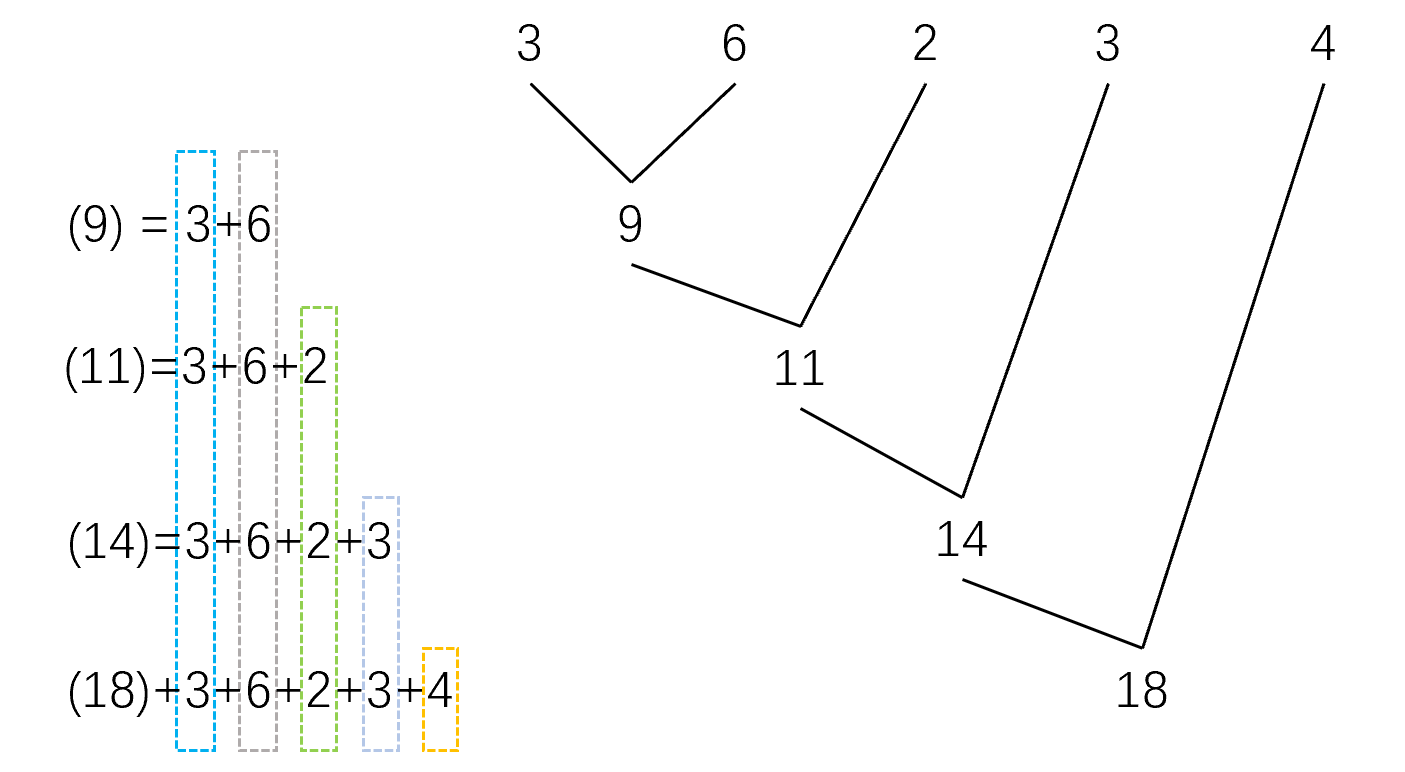
\includegraphics[width=0.7\textwidth]{assets/pics_and_ppts/ch4/柴薪的合并过程.png}
    \caption{柴薪的合并过程}
    \label{fig:柴薪的合并过程}
\end{figure}

可以看出，一堆柴薪参与合并后，并不会从后续的合并过程中消失，而是会作为新柴薪的一部分，继续参与后续合并。
例如，初始重量为 3 的柴薪与重量为 6 的柴薪合并后，形成一堆重量为 \(9=3+6\) 的柴薪。虽然新柴薪的重量变成了 9，
但其中仍然包含原来重量为 \uline{3} 的柴薪（9=\uline{3}+6嘛）。因此，当这堆重量为 9 的柴薪再次参与合并时，产生的消耗中仍然包含原来那 3 的重量。也就是说：
\textbf{每堆\uline{原始}柴薪在每次参与合并时，都会为总体力消耗贡献一次自己的初始重量。}于是，若初始重量为 \(w_i\) 的柴薪参与了 \(k_i\) 次合并，
那么它对总消耗的贡献就是 \(w_i k_i\)。因此，整个合并过程的总消耗可以表示为
\[
W=\sum_{i=1}^{n}w_i k_i
\]

另一方面，由图\ref{fig:柴薪的合并过程}可以看出，原始柴薪越靠后参与合并，其总共参与的合并次数就越小，如4只参与了1次合并，而3和6却参与了4次合并。因此，自然要将原始重量
更大的柴薪放在更后面合并，这样其参与的合并次数就小，因而总体造成的体力消耗就更小。

基于以上讨论，很容易设计出最优的合并方案：每次从当前所有柴薪中，选出两堆重量最小的进行合并，直至最后合并完成。对于3, 6, 2, 3, 4这五堆柴薪，一种最优的合并
方式如图\ref{fig:柴薪的最优合并方式}所示。

\begin{figure}[htbp]
    \centering
    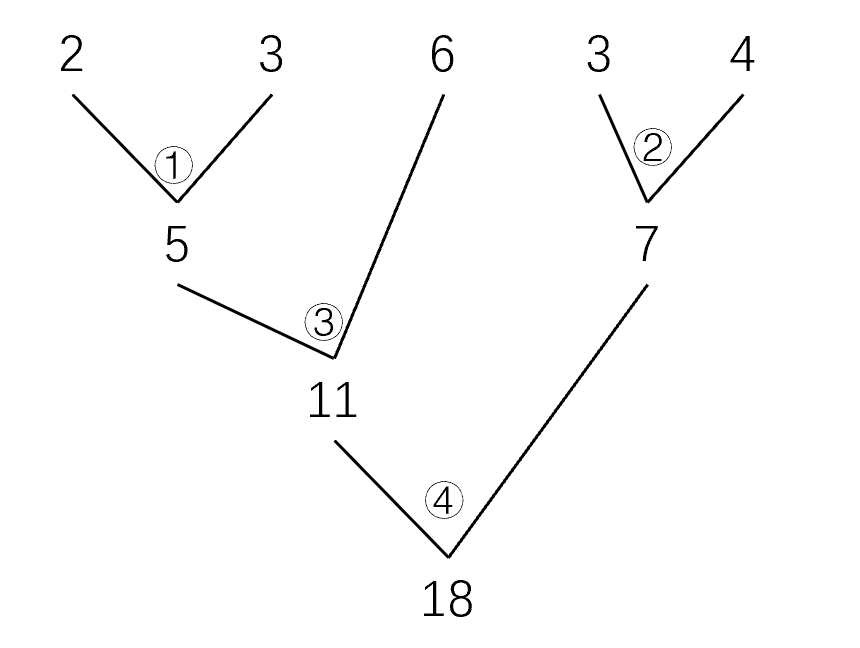
\includegraphics[width=0.45\textwidth]{assets/pics_and_ppts/ch4/柴薪的最优合并过程.png}
    \caption{最优合并过程}
    \label{fig:柴薪的最优合并方式}
\end{figure}
第\Circled{1}步，将最小的2和3合并，消耗体力5，合并后新的柴薪：
\[
    [5, 6, 3, 4]
\]
第\Circled{2}步，将这四堆中最小的3和4合并，消耗体力7，合并后新的柴薪：
\[
    [5, 6, 7]
\]
第\Circled{3}步，将最小的5和6合并，消耗体力11，合并后新的柴薪：
\[
    [11, 7]
\]
第\Circled{4}步，将最小的(也是仅剩的)11和7合并，消耗体力18，合并成最终的一堆柴薪：18。
可以看出，消耗的总体力 = 5 + 7 + 11 + 18 = 41。换个角度，2、3贡献了3次自己的初始重量、6贡献了2次，3和4贡献了2次，因此
$ W=\sum_{i=1}^{n}w_i k_i = (2+3)*3 + 6*2 + (3+4)*2 = 41 $。

相信你早已看出来了，合并的过程其实就构成了一棵二叉树，原始的五堆柴薪就是五个叶子节点，而每堆初始柴薪参与的合并次数$k_i$就是该叶子节点到根节点的\term{路径长度}。
在以上二叉树中，每个节点的数值代表了要搬动这堆柴薪需要消耗的体力。事实上在许多应用中都要类似现象，我们在许多场景下会将树中的节点赋予一个表示某种意义的数值，
称为节点的\term{权}。从树根到一个节点的路径长度与该节点上权值的乘积，就叫做\uline{该节点的}\term{带权路径长度(WPL)}（可以理解为这堆柴薪在后续合并
过程中还会贡献的总体力消耗），而树中所有\uline{叶子节点}的带权路径长度之和就称为\uline{这棵树的}\term{带权路径长度(WPL)}，记为。
\[
\text{WPL}=\sum_{i=1}^{n}w_i k_i
\]
其中$w_i$是第$i$个叶节点的权值，$k_i$是该叶节点到根节点的路径长度。在含有$n$个带权叶节点的二叉树中，带权路径长度最小的二叉树就称为\term{哈夫曼树}。可以看到
在该定义下，“合并柴薪”的问题其实就是求以这n堆柴薪为叶节点的哈夫曼树，其带权路径长度是多少。

通过这个例子，我们也理解了“带权路径长度”以及哈夫曼树的应用价值。图\ref{fig:柴薪的最优合并方式}所示的过程其实也就是由给定的若干个节点，构造一棵哈夫曼树的过程。这里
将该过程完整地叙述如下：
\begin{enumerate}
    \item 初始化。 根据给定的 \(n\) 个权值，构造 \(n\) 棵仅包含一个节点的二叉树，每个节点的权值分别为 \(w_1,w_2,\ldots,w_n\)。
    此时，每棵树都只有一个根节点，且该节点同时也是叶节点。
    \item 选择与合并。 从当前所有二叉树中，选择根节点权值最小的两棵二叉树，将它们合并为一棵新的二叉树。具体而言，
    以一个新节点作为根节点，将选出的两棵二叉树分别作为新根节点的左、右子树，并将新根节点的权值设置为这两棵树的根节点权值之和。
    \item 更新集合。 将刚刚合并得到的新二叉树加入当前的二叉树集合，同时从集合中移除原先被合并的两棵二叉树。这样，集合中的二叉树数量便减少一棵。
    \item 重复执行步骤 2 和步骤 3，直到当前集合中只剩下一棵二叉树。
    \item 得到哈夫曼树。 最终剩下的二叉树就是所构造的哈夫曼树。其所有叶节点的带权路径长度之和最小。
\end{enumerate}

需要注意的是，选择权值最小的两棵树进行合并时，若存在权值相同的节点，可以任选符合条件的两棵树。不同的选择可能构造出形态不同的哈夫曼树，但所得的最小带权路径长度相同。

\minisection{哈夫曼树的性质}
\label{minisec:哈夫曼树的性质}
从以上哈夫曼树的构造过程可以看出哈夫曼树具有如下特点：
\begin{enumerate}
    \item 最初有$n$个叶节点，合并需要$n-1$步，因此新增共$n-1$个节点。所以：\textbf{具有$n$个叶节点的哈夫曼树，其总结点数一定是$n+n-1=2n-1$}。
    \item 所有有孩子的节点一定都是由2棵子树合并而来，因此\textbf{哈夫曼树中不存在度为1的节点}。
\end{enumerate}
这两条性质在某种角度其实是相通的。

\subsection{哈夫曼编码}
我们知道数字信号是一种二值信号，通过有不同特征的电信号来表示0或1。将字符编码成二进制信号，就可以实现数字信号的传输。如最经典的ASCII编码，
\textquotesingle A\textquotesingle 的编码为65，传输过程中的数字信号为 01000001，而\textquotesingle a\textquotesingle 对应的数字信号为 01100001。
这种编码方式是\term{等长编码}，对所有字符的编码长度相等，都是8位，都需要8个bit。
但是，实际应用中，各个字符的使用率却大有差异。例如一篇新闻报道中，\textquotesingle e\textquotesingle 和\textquotesingle \; \textquotesingle（空格）
等字符的数量一定远大于\textquotesingle \$\textquotesingle 和\textquotesingle x\textquotesingle 等字符。

显然，如果我们能够将出现频率更高的字符编码得更短，而频率低的字符编码较长，就可以减少所需的传输空间。

然而这种\term{不定长编码}也带来了一个新的问题：
对方收到之后，如何解码？比如你将A、B、C分别编码为0、1、01，那么收到0101，应解码为ABAB还是ABC或CC？

因此，我们还需要为编码方案增加一个重要的约束：\textbf{任何一个字符的编码，都不能是另一个字符编码的前缀}。满足这一条件的编码称为\term{前缀编码（Prefix Code）}。

\begin{insightbox}
    在诸多英文文献中，\term{前缀编码（Prefix Code）}也被称为“Prefix-free Code”，即“无前缀编码”。笔者认为后者在语义上更加直观。
\end{insightbox}

于是问题就变成了：给定n个字符$c_1, c_2, ..., c_n$及它们的权重（即字符出现的次数）$w_1, w_2, ..., w_n$，求一种前缀编码方案让总编码长度达到最小。

我们可以借助二叉树来解决这样的编码问题。我们规定从根节点向左走代表数字 $0$，向右走代表数字 $1$。如图\ref{fig:用二叉树进行不定长编码}所示，
这样，从根节点到任意节点的路径，就可以用一串二进制数字表示。如果我们将每个字符放在一片叶节点上，那么从根节点到该叶节点的路径，就可以作为这个
字符的编码，路径长度也即是编码长度。该例中，A的编码为000，到根节点的路径长度为3，即是编码长度；B的编码为01，路径长度、编码长度为2；C的编码为1。

\begin{figure}[htbp]
    \centering
    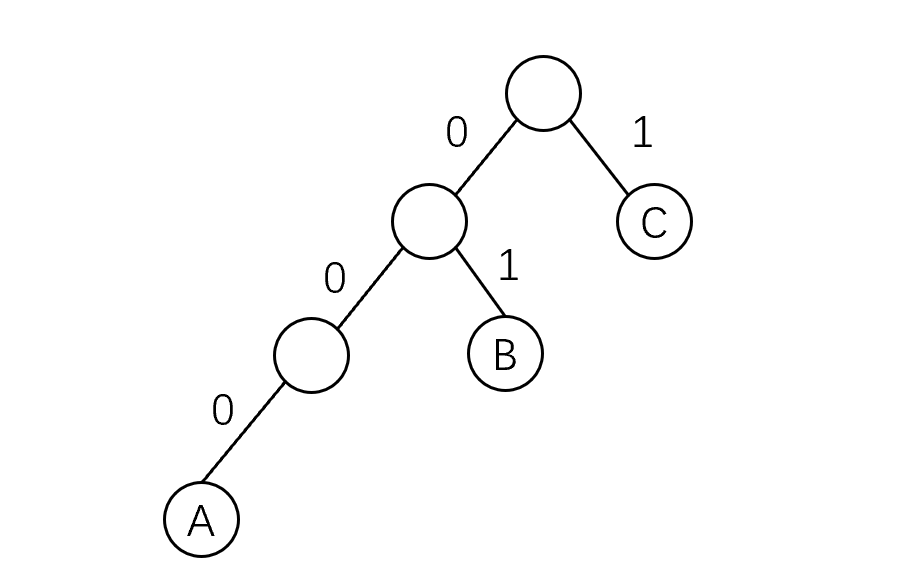
\includegraphics[width=0.47\textwidth]{assets/pics_and_ppts/ch4/用二叉树进行不定长编码.png}
    \caption{用二叉树进行不定长编码}
    \label{fig:用二叉树进行不定长编码}
\end{figure}

假设字符 $c_i$ 出现的次数为 $w_i$，其在二叉树中对应叶节点的深度为 $k_i$，
则传输所有字符所需的总比特数为
\[
    L=\sum_{i=1}^{n} w_i k_i
\]
而这恰好就是该树的带权路径长度（WPL）。因此，在字符及其出现次数固定的情况下，使总编码长度最小，等价于使二叉树的带权路径长度最小。因此求解该问题，实际上就是
构造哈夫曼树的过程。例如，A, B, C, D, E五个字符出现次数依次是3, 6, 2, 3, 4，则可以构造如图\ref{fig:哈夫曼编码}所示的哈夫曼树。
\begin{figure}[htbp]
    \centering
    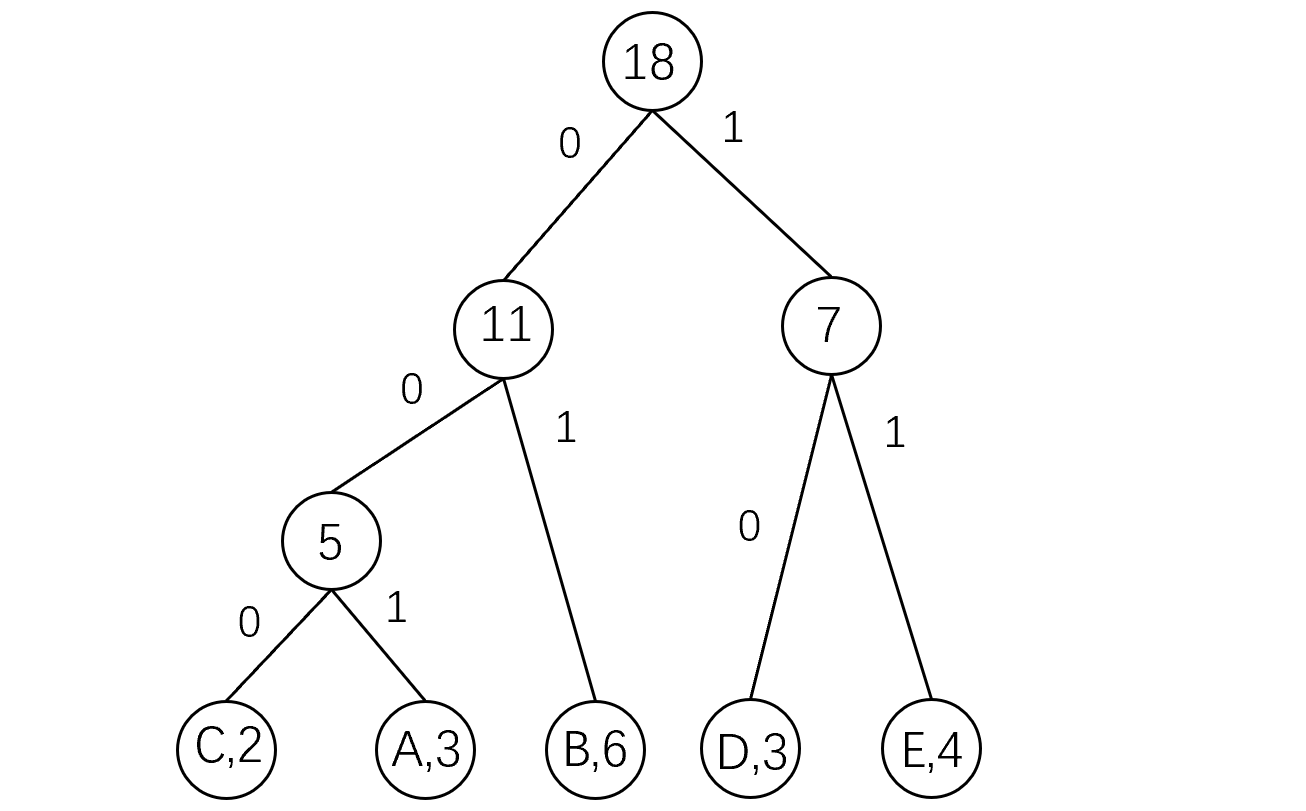
\includegraphics[width=0.5\textwidth]{assets/pics_and_ppts/ch4/哈夫曼编码.png}
    \caption{哈夫曼编码}
    \label{fig:哈夫曼编码}
\end{figure}

A、B、C、D、E的编码与长度如下：
\begin{center}
    \begin{tabular}{|c|c|c|}
        \hline
         & 编码值 & 编码长度/路径长度\\
        \hline
        A & 001 & 3\\
        \hline
        B & 01 & 2\\
        \hline
        C & 000 & 3\\
        \hline
        D & 10 & 2 \\
        \hline
        E & 11 & 2 \\
        \hline
    \end{tabular}
\end{center}

同时，由于叶节点不可能是其他节点的祖先，因此，任何一个字符的编码都不会成为另一个字符编码的前缀。这恰好满足了前缀编码的要求。这种由哈夫曼树产生的编码称为
\term{哈夫曼编码}。显然对于相同字符集存在多种哈夫曼编码，但它们的编码长度是相同的。

\begin{notebox}{提示}
    当然，你也可以将向左定义为1，向右定义为0。类似的思想已经提示过多次，此处是最后一次了，我保证。
\end{notebox}

\vspace{1em}
在“合并柴薪”问题中，一堆柴薪参与合并的次数越多，它的重量就会在总代价中被累加越多次；在“字符编码”问题中，一个字符的编码越长，它消耗的传输空间就越多。
二者共同的底层逻辑是：\textbf{每个对象都有自己的权值，而我们可以通过不同的安排，决定这个权值会被计入最终结果多少次。}

\begin{thinkbox}
    对于“合并柴薪”问题，你能否写出一个函数，输入一组重量，输出最优的体力消耗值（只要输出这个数值就行）？
\end{thinkbox}
通过上面的思考你也许会发现，解决此类问题并不需要真的构造出一棵哈夫曼树。编码问题亦是如此，同样不需要在计算机中存储哈夫曼树。事实上，哈夫曼树的意义在于，对于这类问题，
它为我们提供了统一的数学模型和统一的求解方法。

还有一个问题，以“合并柴薪”问题为例，我们需要每次从当前所有柴薪堆中选出两个重量最小的，合并后再放回去。使用什么数据结构保存柴薪堆，能使这个操作达到最快？显然若使用普通线性表，
对于频繁插入删除的场景，链表一定更好。选择两个最小、合并后再插入的时间可以达到O(n)。

我们在接下来的介绍中将看到，如果使用\term{堆}保存所有柴薪的重量，这个选择加合并后插入的过程可以达到O(logn)。如果你熟悉C++，应该已经想到了使
用一个std::priority\_queue来保存所有柴薪堆，实际上，C++标准库中的priority\_queue正是通过\term{堆}来实现的。

\section{堆}
\term{堆}是一棵完全二叉树，满足其中任何一个节点的关键字的值都不大于（或不小于）其左右子树中任何一个节点的关键字的值。完全二叉树的根节点称为\term{堆顶}。若任何一个节点的值都不
大于其左右子树，这样的堆叫做\term{最小堆}，也叫\term{小顶堆}或\term{小根堆}，堆顶元素一定是堆中最小的；若任何一个节点的值都不小于其左右子树，
这样的堆叫做\term{最大堆}，也叫\term{大顶堆}或\term{大根堆}，堆顶元素一定是堆中最大的。图\ref{fig:最小堆和最大堆}
（左）和（右）分别展示了一个最小堆和一个最大堆。
\begin{figure}[htbp]
    \centering
    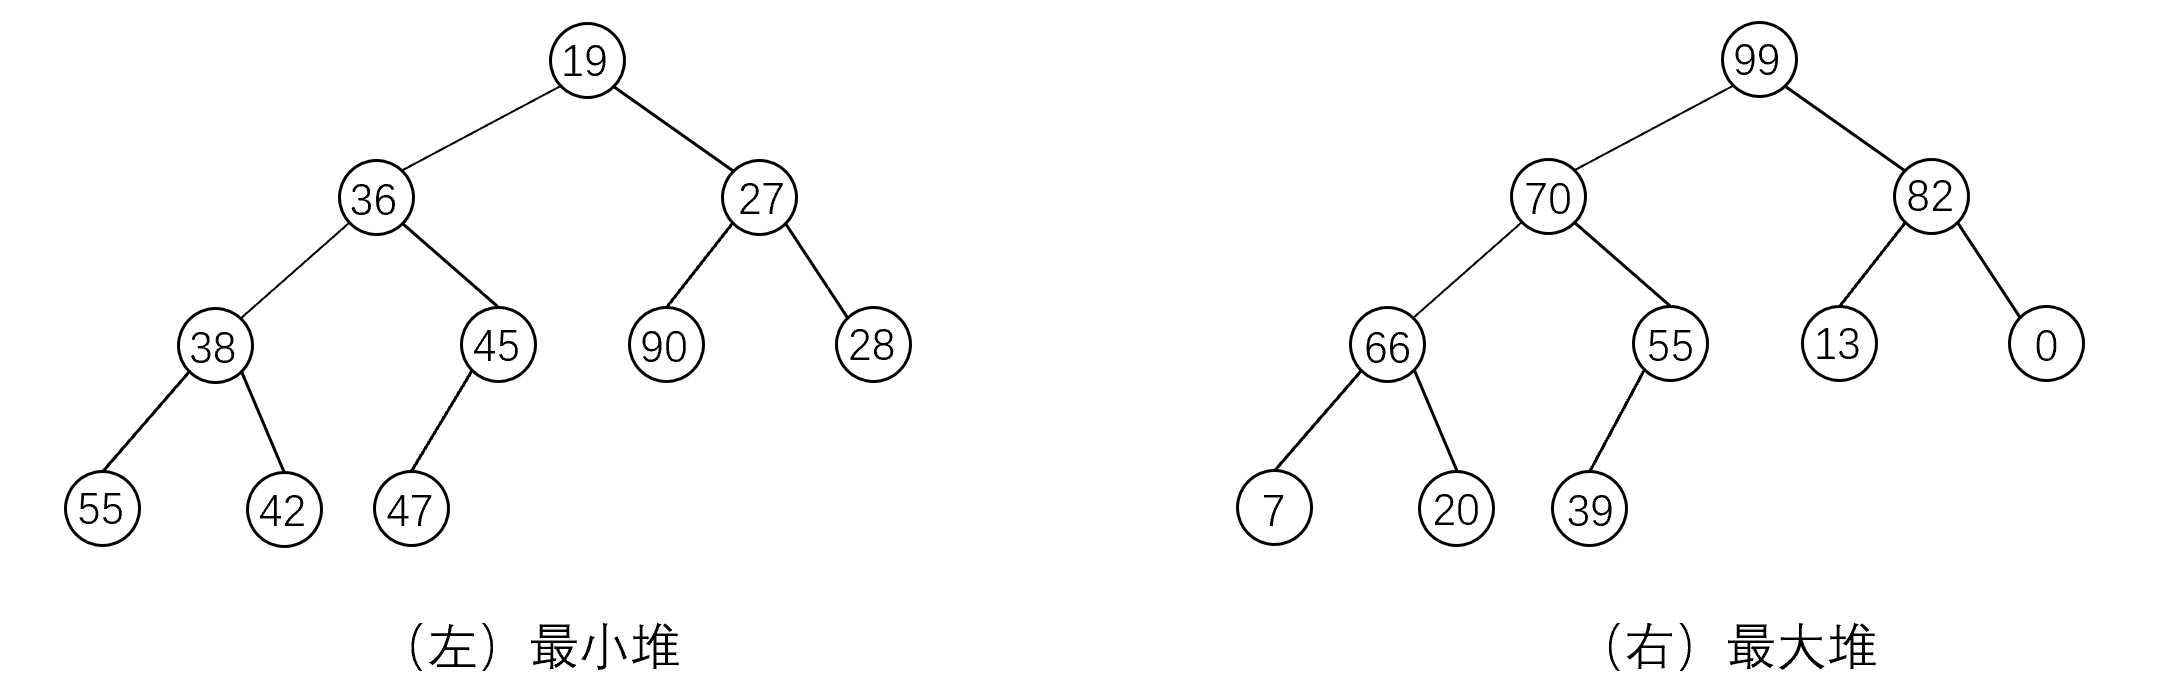
\includegraphics[width=0.81\textwidth]{assets/pics_and_ppts/ch4/最小堆和最大堆.png}
    \caption{}
    \label{fig:最小堆和最大堆}
\end{figure}

请注意：以最大堆为例，最大堆能保证：
\Circled{1}根节点一定是最大的；\;
\Circled{2}任何一个节点，都比其左右子树中的节点大。\;但是最大堆无法保证上层节点一定大于下层节点，因为它们不一定处于同一棵子树中。如图\ref{fig:最小堆和最大堆}（右）中，节点39虽处于第4层，但它比第3层的13、0还要大。

\begin{insightbox}
    关键字（Key）可以理解为用于标识数据或确定数据比较关系的一个或多个数据项。 在排序等问题中，通常根据关键字的值来确定数据的大小关系。例如，对于字符
    数据，可以将其 ASCII 码值作为关键字；对于游戏中的武器数据，可以将武器的id或攻击力作为关键字。
\end{insightbox}

\subsection{堆及其常见操作的实现}
由于堆是一棵完全二叉树，因此用一个数组顺序存储就非常合适（参见\ref{minisec:二叉树的顺序存储}，第\pageref{minisec:二叉树的顺序存储}页）。
使用数组存储一个堆也是最常见、最方便的实现方式。通常情况下通过一个数组和一个整数，就可以表示一个堆：
\begin{cppcode}
    int heap[MaxSize+1];
    int size = 0;  // 堆中元素的数量
\end{cppcode}
注意我们定义根节点编号为1，从数组下标1开始存储。显然这种存储方式下，heap[1]就能获取堆顶元素的值，时间复杂度为O(1)。

为了方便大家建立对堆的感觉，我们先来看如何将一个已有若干元素的完全二叉树（数组存储）调整成一个堆。本节所有对堆操作的介绍均以\uline{最大堆}为例。
假设数组arr[]中已经存储了完全二叉树的n个节点，可以通过如下操作将这个完全二叉树调整成一个堆：
\minisection{将完全二叉树调整为堆}
从编号为$ \left \lfloor \frac{n}{2} \right \rfloor $ 的节点，即最后一个非叶子节点开始，逐一向前检查每一个节点，对每个节点
进行\term{向下调整}操作。将节点\term{向下调整}是指，将该节点与其两个孩子（若存在）中较大的那个比较，若该节点小于较大的那个孩子，
则将该节点“下沉”，与较大的那个孩子交换位置。交换后，该节点到了新的位置，继续检查能否继续“下沉”，直到该节点沉入某个无法继续与孩子
交换的位置，或沉到叶节点。我们以图\ref{fig:建堆操作初始树}所示的完全二叉树为例，介绍详细的流程。
\begin{figure}[htbp]
    \centering
    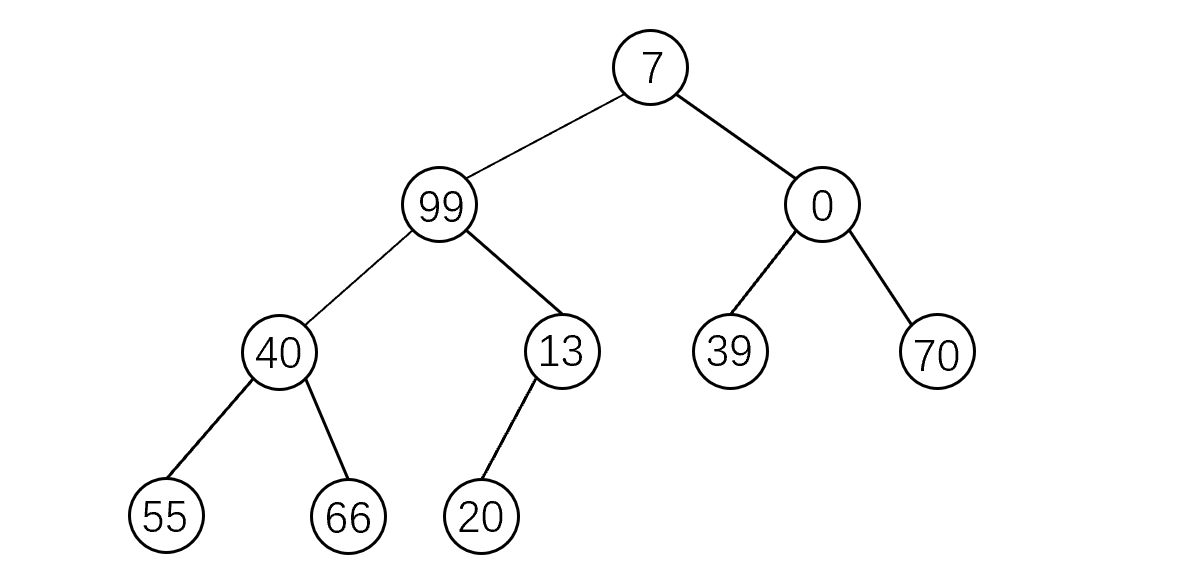
\includegraphics[width=0.59\textwidth]{assets/pics_and_ppts/ch4/建堆操作初始树.png}
    \caption{}
    \label{fig:建堆操作初始树}
\end{figure}    

该树共有10个节点，第一个非叶子节点编号为$ \left\lfloor \frac{10}{2} \right\rfloor = 5$，因此我们逐个检查编号为5、4、3、2、1的节点，尝试将它们下沉。\\
\Circled{1} 如图\ref{fig:建堆流程-1}，检查节点13， 它只有一个左孩子，因此与其左孩子比较，发现左孩子更大，所以交换。交换后，13已经沉到底。继续检查下一个节点；\\
\begin{figure}[htbp]
    \centering
    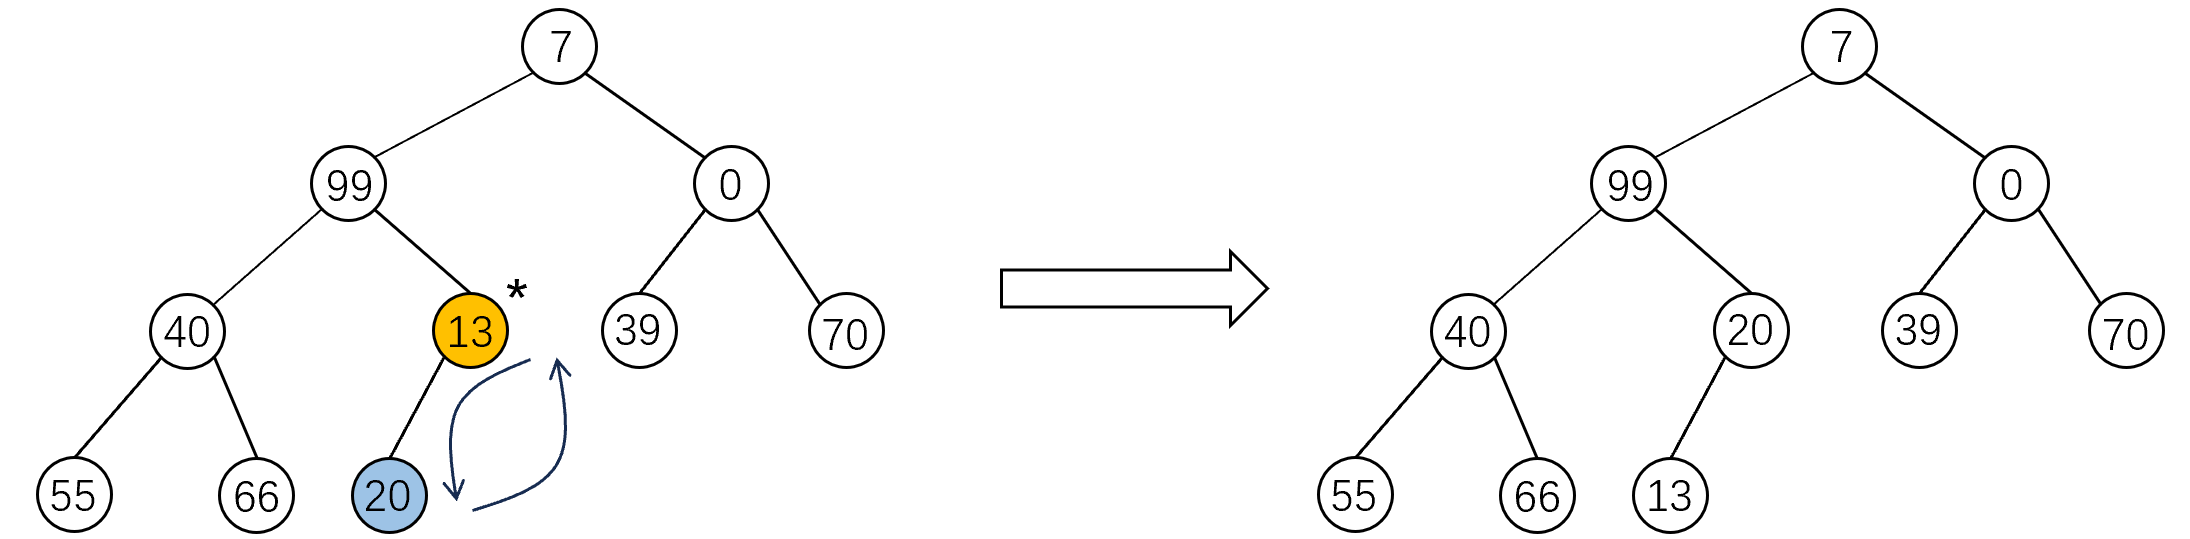
\includegraphics[width=0.88\textwidth]{assets/pics_and_ppts/ch4/建堆流程-1.png}
    \caption{}
    \label{fig:建堆流程-1}
\end{figure}
\Circled{2} 如图\ref{fig:建堆流程-2}，检查节点40，它有两个孩子节点，其中右孩子66较大，因此将该节点40与右孩子66进行比较，该节点小于右孩子，于是下沉；\\
\begin{figure}[htbp]
    \centering
    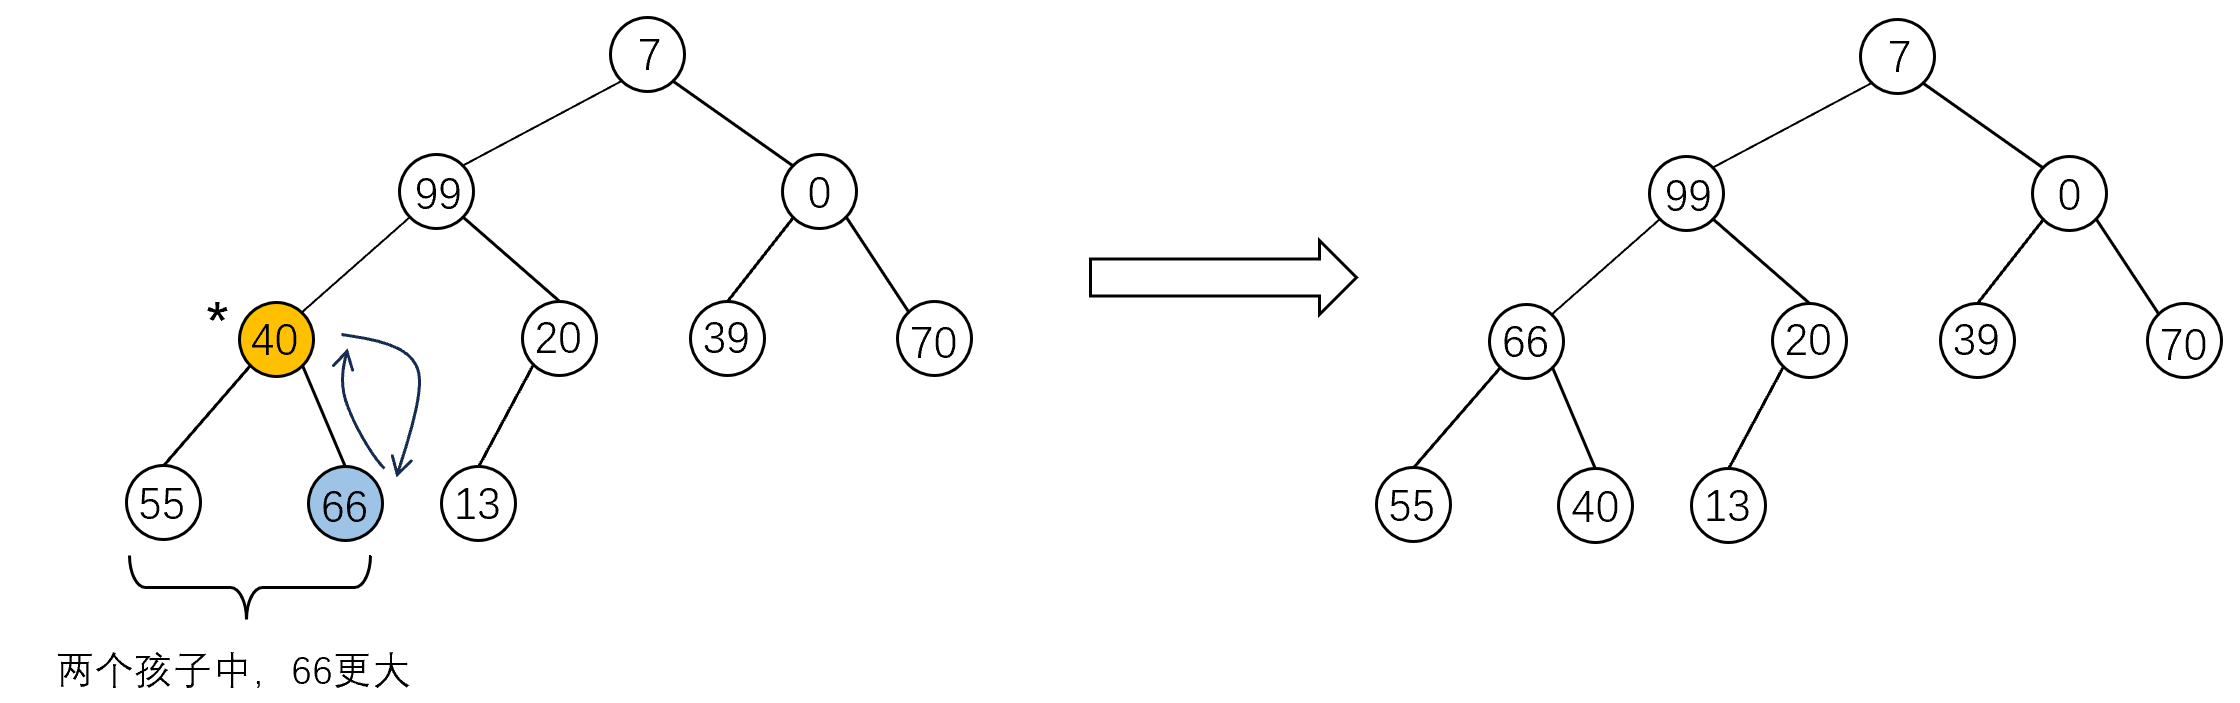
\includegraphics[width=0.88\textwidth]{assets/pics_and_ppts/ch4/建堆流程-2.png}
    \caption{}
    \label{fig:建堆流程-2}
\end{figure}
\Circled{3} 如图\ref{fig:建堆流程-3}，检查节点0，它有两个孩子，其中右孩子70较大，因此将该节点0与右孩子70进行比较，该节点小于右孩子，于是下沉。已沉底，继续
检查下一个节点。\\
\begin{figure}[htbp]
    \centering
    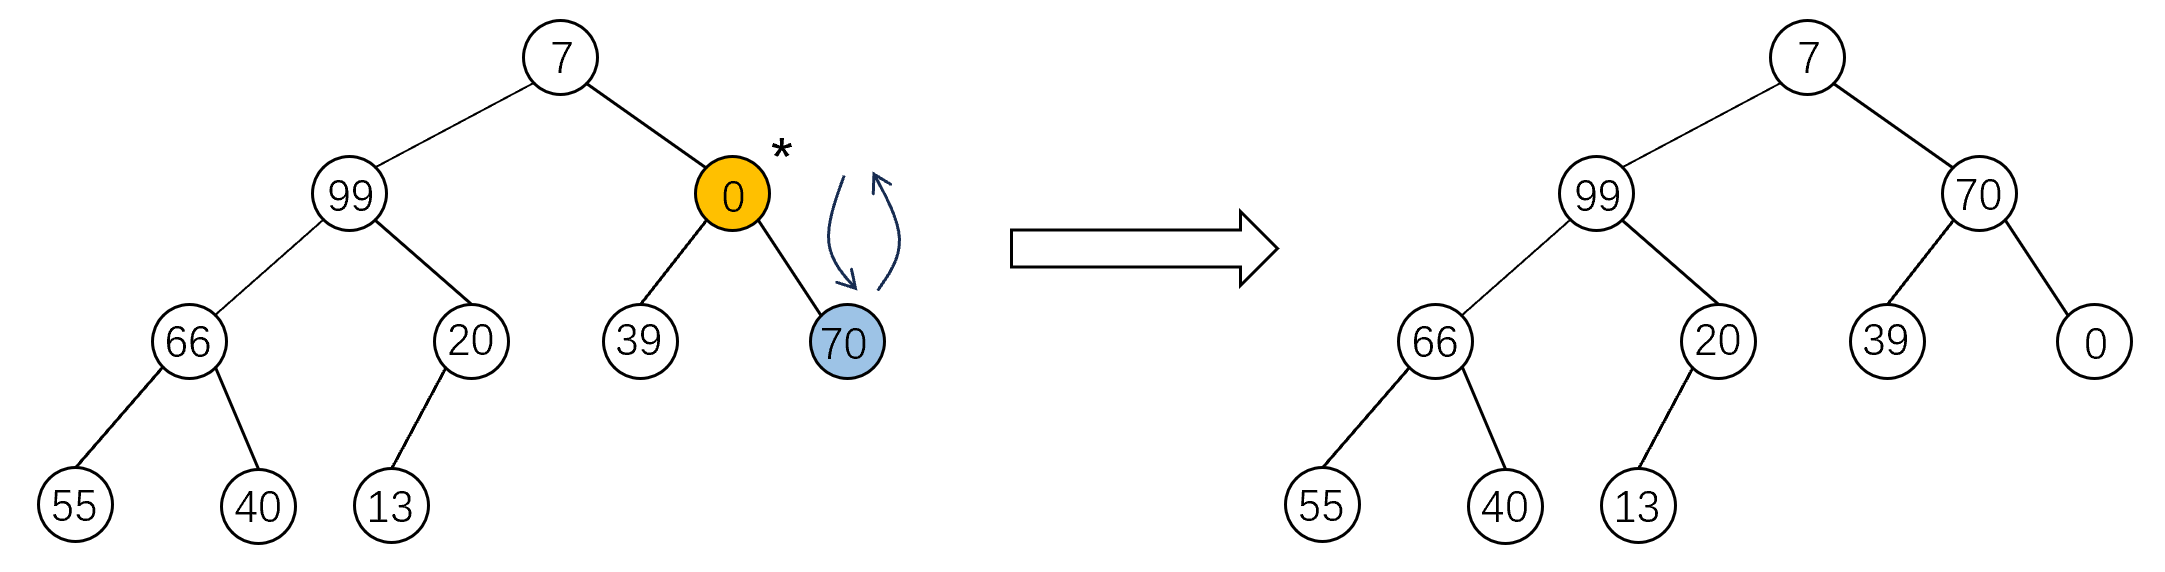
\includegraphics[width=0.88\textwidth]{assets/pics_and_ppts/ch4/建堆流程-3.png}
    \caption{}
    \label{fig:建堆流程-3}
\end{figure}
\Circled{4} 如图\ref{fig:建堆流程-4}，检查节点99，它有两个孩子，其中左孩子66较大，因此将该节点99与左孩子66进行比较，该节点不小于66，无需调整，继续检查下一个
节点。\\
\begin{figure}[htbp]
    \centering
    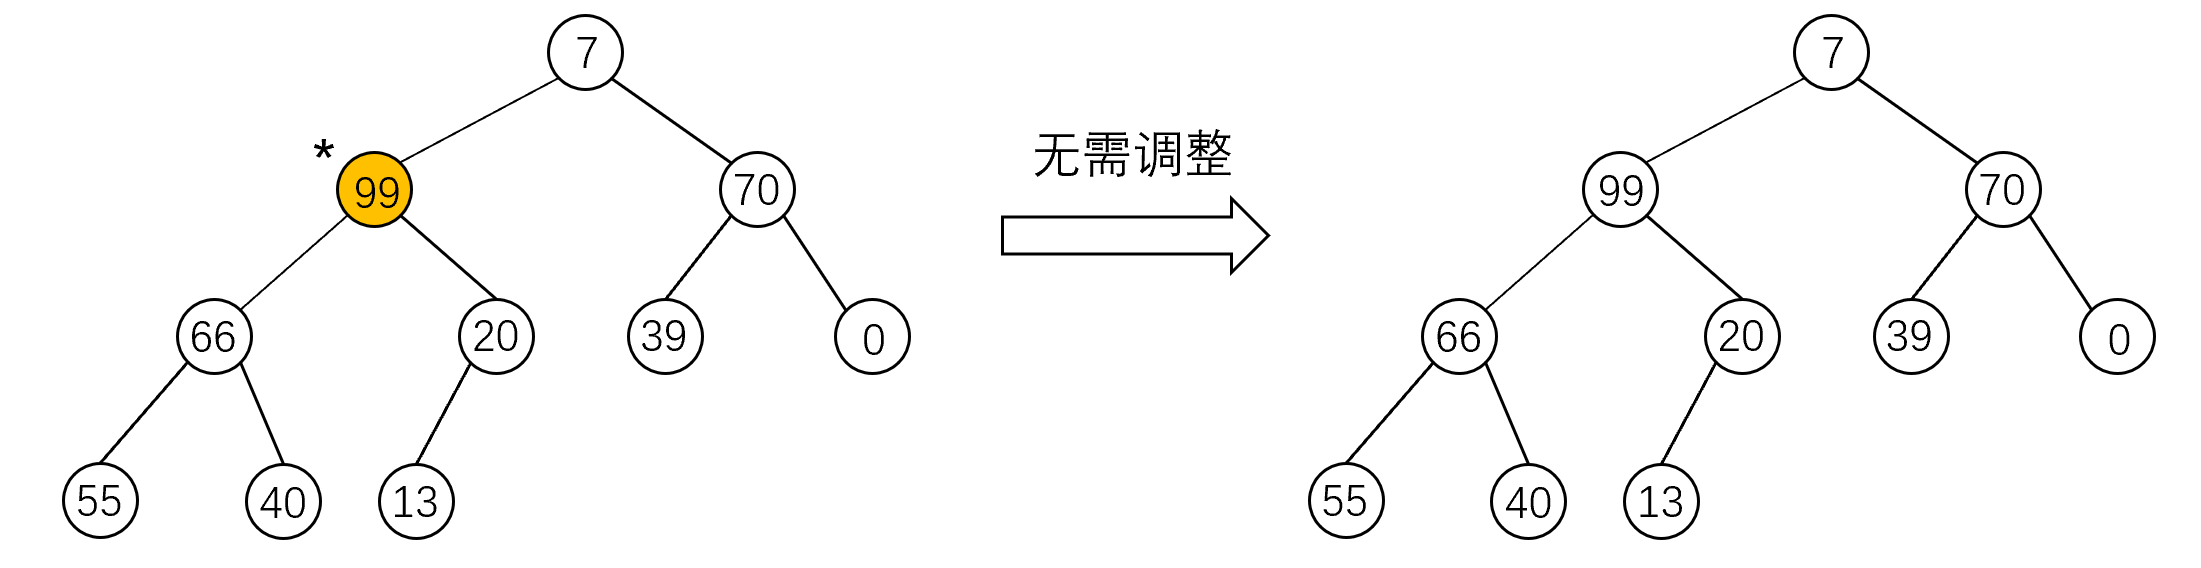
\includegraphics[width=0.88\textwidth]{assets/pics_and_ppts/ch4/建堆流程-4.png}
    \caption{}
    \label{fig:建堆流程-4}
\end{figure}
\Circled{5} 如图\ref{fig:建堆流程-5}，检查节点7，它有两个孩子：99和70，因此7与99交换；交换后继续判断7是否应该继续下沉：此时7的两个孩子分别是66和20，与66
比较，7比66小，继续和66交换位置；之后继续和两个孩子中较大的55比较，小于55，和55交换，到达叶子节点，节点7的向下调整完成。\\

经过了上述过程，堆就已经建好了。
\begin{figure}[htbp]
    \centering
    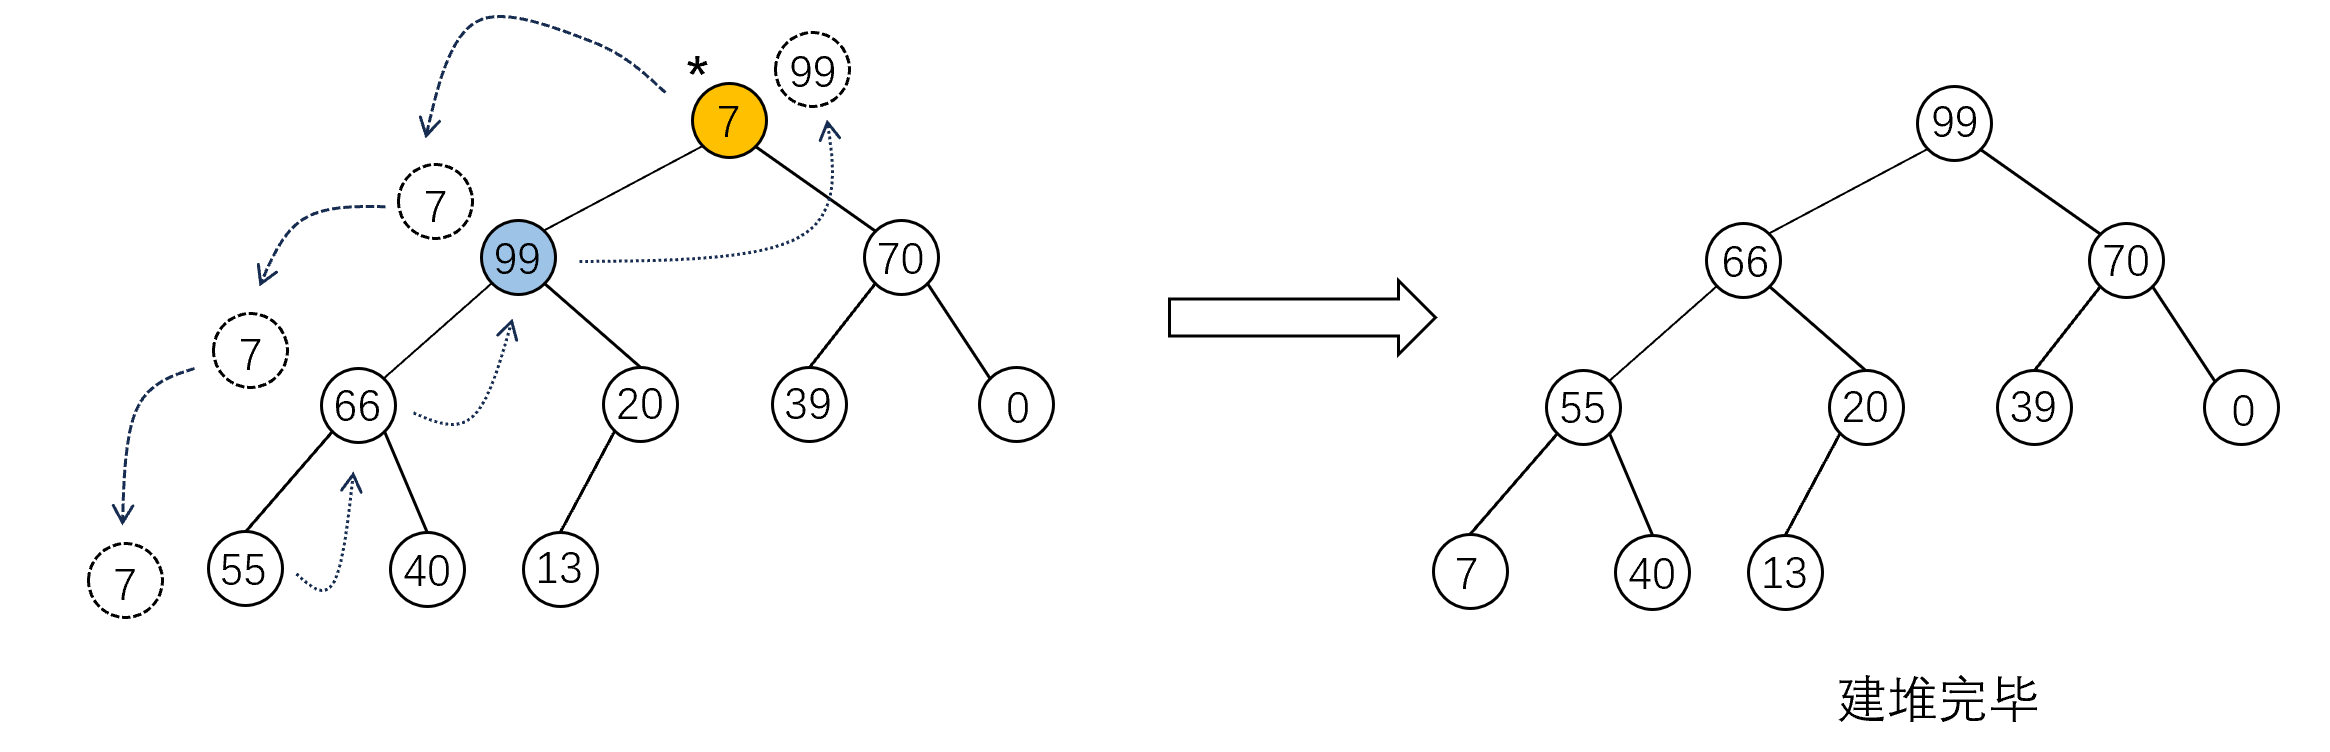
\includegraphics[width=0.88\textwidth]{assets/pics_and_ppts/ch4/建堆流程-5.png}
    \caption{}
    \label{fig:建堆流程-5}
\end{figure}
从一个已有的完全二叉树建堆的过程如代码\ref{code:堆的向下调整及建堆代码}所示。注意在向下调整的函数DownAdjust()中，while循环终止有两种可能，一是2*i 已经大于 n 了，
即该节点已经调整到了叶子节点，没有孩子了；二是该节点已经调整到了某位置，其值不小于两个孩子中更大的那个了，无需继续下沉。
\begin{cppcodeNum}[label={code:堆的向下调整及建堆代码}, codetitle={堆的向下调整及建堆代码}]
// 元素数量为n的完全二叉树中，将编号为 i 的元素向下调整
    void DownAdjust(int arr[], int n, int i) {
        // i表示下沉过程中，该节点已经“沉入”到了编号为多少的地方。
        // 最后一个节点编号是n，因此2*i<=n表示该位置还有子节点
        while(2*i <= n) {
            int max_child = arr[2*i];   // 先假设左孩子是更大的
            int max_child_idx = 2*i;
            // 事实上右孩子存在，且右孩子更大
            if(2*i+1 <= n && arr[2*i+1] > arr[2*i]) {
                max_child = arr[2*i+1]; 
                max_child_idx = 2*i+1;
            }
            // 该元素较小，应该继续下沉 
            if(arr[i] <= max_child) {
                int t = arr[i];
                arr[i] = arr[max_child_idx];
                arr[max_child_idx] = t;
                i = max_child_idx;
            } 
            // 已经不满足继续下沉的条件，向下调整完成。
            else {
                break;
            }
        } 
    }
// 将具有n个元素，存储在arr[]数组中的完全二叉树调整成一个堆。
    void CreateHeap(int arr[], int n){
        for(int i=n/2; i>=1; i--) {
            DownAdjust(arr, n, i);
        }
    }
\end{cppcodeNum}
向下调整，至多需要“下沉”约logn次，时间复杂度为O(logn)。而对于建堆操作，需要将约n/2个元素向下调整，每个元素向下调整的时间复杂度为O(logn)，那整个
建堆过程就是O(nlogn)。
\begin{thinkbox}
    可是，建堆过程是O(nlogn)这个说法真的是正确的吗？\\

    这里我只给出正确的说法：建堆操作的时间复杂度应该是O(n)，而非O(nlogn)。这是一个很有意思的问题。大家可以从直观上想一想为什么。
    严谨的证明过程较复杂，感兴趣的同学可以参考《算法导论》。
\end{thinkbox}

\minisection{向上调整、向堆中插入元素}
要往堆中加入一个元素，可以先将该元素放在数组尾部（即完全二叉树的最后一个节点后面），再将该元素\term{向上调整}。与向下调整类似，\term{向上调整}就是将该节点
不断地与其父节点比较，若大于父节点，则将该节点“上浮”，与父节点交换位置，之后不断重复该操作，直至不满足上浮条件，或已经上浮到根节点，如此，该节点的向上调整
就完成了。向上调整与插入操作的代码实现如\ref{code:向上调整及插入操作}所示。

\begin{cppcodeNum}[label={code:向上调整及插入操作}, codetitle={向上调整及插入操作}]
// 元素数量为n的完全二叉树中，将编号为 i 的元素向上调整
    void UpAdjust(int arr[], int n, int i) {
        // i表示上浮过程中，该节点已经上浮到了编号为多少的地方。
        while(i/2 > 0) {    // 此位置还有父节点
            int father_idx = i/2;
            if(arr[i] > arr[father_idx]) {
                int t = arr[i];
                arr[i] = arr[father_idx];
                arr[father_idx] = t;
                i = i/2;
            }
            else {
                break;
            }
        }
    }
    // 向当前有n个元素的堆arr中，插入新元素e
    void InsertHeap(int arr[], int& n, int e) {
        n += 1;
        arr[n] = e;
        UpAdjust(arr, n, n);
    }
\end{cppcodeNum}
与向下调整类似，向上调整的时间复杂度同样为O(logn)。显然插入操作的时间复杂度也是O(logn)。

\begin{notebox}{提示}
    如果为了更加能体现出数组表示的数据结构是一个堆，可以将一个数组以及堆中当前元素数量进行一个封装：
    \begin{cppcode}
    #define MaxSize 100
        struct Heap {
            int arr[MaxSize+1];
            int n;  // 堆中当前元素数量
        };
    \end{cppcode}
    这样，相关操作的接口语义会更加明确一些：
    \begin{cppcode}
        void UpAdjust(Heap& h, int i);  // 将堆h中编号为i的元素向上调整
        void InsertHeap(Heap& h, int e); // 向堆h中插入一个新元素e
    \end{cppcode}
    等。此外，注意插入操作需考虑堆满的情况，我们在前面介绍过，为将关注重点放在算法的核心思想上，在许多合适的地方我们将省去这些代码，以减轻理解负担。后面将
    不再提及此事。
\end{notebox}

\minisection{删除堆顶元素}
要删除堆顶元素，只要用\term{堆底元素}，即完全二叉树的最后一个节点，覆盖掉堆顶元素，然后将新的堆顶向下调整即可。如代码\ref{code:删除堆顶元素}所示。
\begin{cppcodeNum}[label={code:删除堆顶元素}, codetitle={删除堆顶元素}]
    void DeleteTop(int arr[], int& n) {
        if(n == 0) return ;
        arr[1] = arr[n];
        n -= 1;
        DownAdjust(arr, n, 1);
    }
\end{cppcodeNum}
显然删除堆顶元素的操作时间复杂度为O(logn)。\\

注意以上所有操作都是以最大堆为例来介绍的。最小堆的操作类似。

\subsection{堆的经典应用}
下面介绍一些堆的经典的、最常见的应用场景。
\minisection{1.动态维护最大值或最小值}
堆的一个重要价值在于，能够在数据不断变化时，以 O(logn)的时间复杂度插入和删除元素，并以O(1)的时间复杂度获取当前的最大值或最小值，也就是能高效地动态维护优先级最高的元素。
例如在\ref{sec:哈夫曼树与哈夫曼编码}（第\pageref{sec:哈夫曼树与哈夫曼编码}页）中介绍的“合并柴薪”以及“字符编码”问题，需要不断地从容器中删除两个最小的，合并
之后再插入容器，这种问题非常适合使用堆来实现。

一个比较有趣的事情是，{\color{red}\textbf{在后面的介绍中我们将看到}}，求解最短路径的大名鼎鼎的迪杰斯特拉算法，使用堆可以进一步提升性能。

\minisection{2.找出大量数据中最大或最小的k个}
例如，如果需要从10万件商品中，筛选价格最低的k件商品，最朴素的做法是对这10万件商品遍历k次，第i次遍历找出第i小的价格。但是这需要某种手段标记i之前已经
被找到了的元素。算法时间复杂度为O(nk), 并且需要额外空间。

如果使用排序算法，{\color{red}\textbf{我们将在后面的内容中介绍到}}，最好可以达到O(nlogn)的时间将这10万件商品排成一个有序的列表，再取前k件即可。时间复杂
度为O(nlogn)，空间复杂度最好（堆排序）为O(1)。

一种更巧妙的做法是，我们建立一个具有k个元素的\textbf{最大堆}，保存10万个元素中最小的k个，让这100000个元素“争抢进入这个堆的权利”，谁更小，谁就能进入堆中。
显然，只要某个元素至少小于堆中的某一个元素，该元素即可进入堆中。而事实上对最大堆来说：
\begin{bulk}
    \begin{center}
        至少小于一个元素 => 小于堆顶元素    一定成立\\[0.6em]
        小于堆顶元素 => 至少小于一个元素    一定成立\\[0.6em]
        因此至少小于一个元素 <=> 小于堆顶元素
    \end{center}
\end{bulk}
因此我们逐一检查这100000个元素，将它们依次与堆顶元素进行比较，若小于堆顶元素，说明该元素是当前检查过的所有元素里前k小的，此时若堆已满，令其覆盖堆顶元素并调整堆，
保证堆顶依然是堆中最大的；若堆未满，直接将其加入堆中。直至检查完所有元素，堆中保存的，即是这所有10万个元素中最小的k个元素。

该方法需要对所有n个元素进行一遍访问，每次访问可能需要对堆进行调整，对于有k个元素的堆，调整堆的复杂度为O(logk)，因此整体时间复杂度为O(nlogk)。与排序算法可以达到
的O(nlogn)相比，有所提升。同时该方法需要一个额外的k个空间的辅助堆，空间复杂度为O(k)。

\section{并查集}
\label{sec:并查集}
现在考虑这样一个问题：某个游戏的世界地图上，存在$N$个城镇，编号为$0$到$N-1$，初始时它们彼此之间是不连通的。玩家可能在游玩过程中修建道路，使得两个城镇连通起来。显然对任意的城镇
0、1、2，若0与1连通，1与2连通，则0与2一定连通。不妨将处于同一个\uwave{连通块}中的城镇看成是在同一个集合中，则最初有$N$个不同的集合。

现在假设游戏的玩法规定：仅当两个城镇0和1不连通（不在同一个集合中）时，玩家才可以修建0到1的道路。
如下图a），0与2已经连通了，因此不允许修建道路0->2，而 b）中0与2并未连通。
\begin{center}
    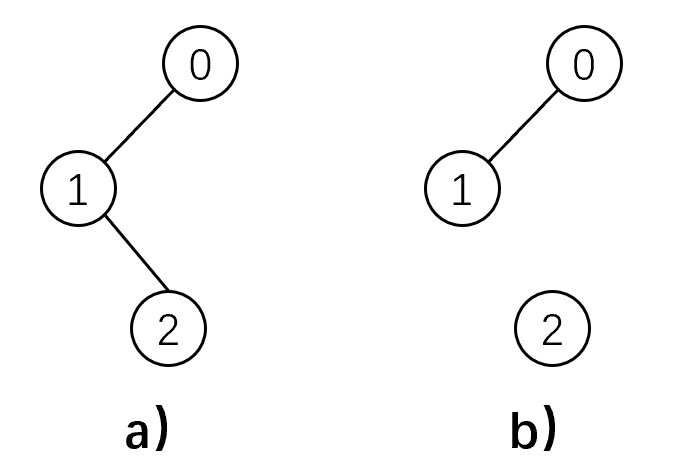
\includegraphics[width=0.31\textwidth]{assets/pics_and_ppts/ch4/并查集连通性说明.png}
\end{center}
因此当玩家尝试修建某条A->B的道路时，程序需要判断A与B是否在同一个集合中，若是，则拒绝玩家的请求；否则，需要将A与B所在的两个集合合并成一个集合。

事实上，在诸多需求中（如，\ref{subsec:Kruskal算法}节中将要介绍的Kruskal算法）都会有类似的需求场景：

1）判断两个元素是否属于同一个集合；

2）将两个不同集合合并为同一个集合。

如何能够高效地实现以上两个操作呢？最直接的思路就是记录每一个元素所属的集合编号，如：
\begin{center}
    \begin{tabular}{ccccc}
        \hline
        城镇 & 0 & 1 & 2 & $\cdots$ \\
        \hline
        集合编号 & 0 & 0 & 2 & $\cdots$ \\
        \hline
    \end{tabular}
\end{center}


这样，判断两个元素是否属于同一个集合只需要比较编号即可：
\begin{cppcode}
    bool SameSet(int a, int b) {
        return id[a] == id[b];
    }
\end{cppcode}
查询操作非常简单，时间复杂度为 \(O(1)\)。但是，当集合合并时，就要将其中一个集合的所有元素编号都改为另一个集合的编号，若集合元素非常多，
则需要大量修改。这种设计查询很快，但合并可能很慢。

事实上，这种设计可以这样理解，将每个集合中其中一个元素的编号作为该集合的编号，如下图a）所示的两个集合：
\begin{center}
    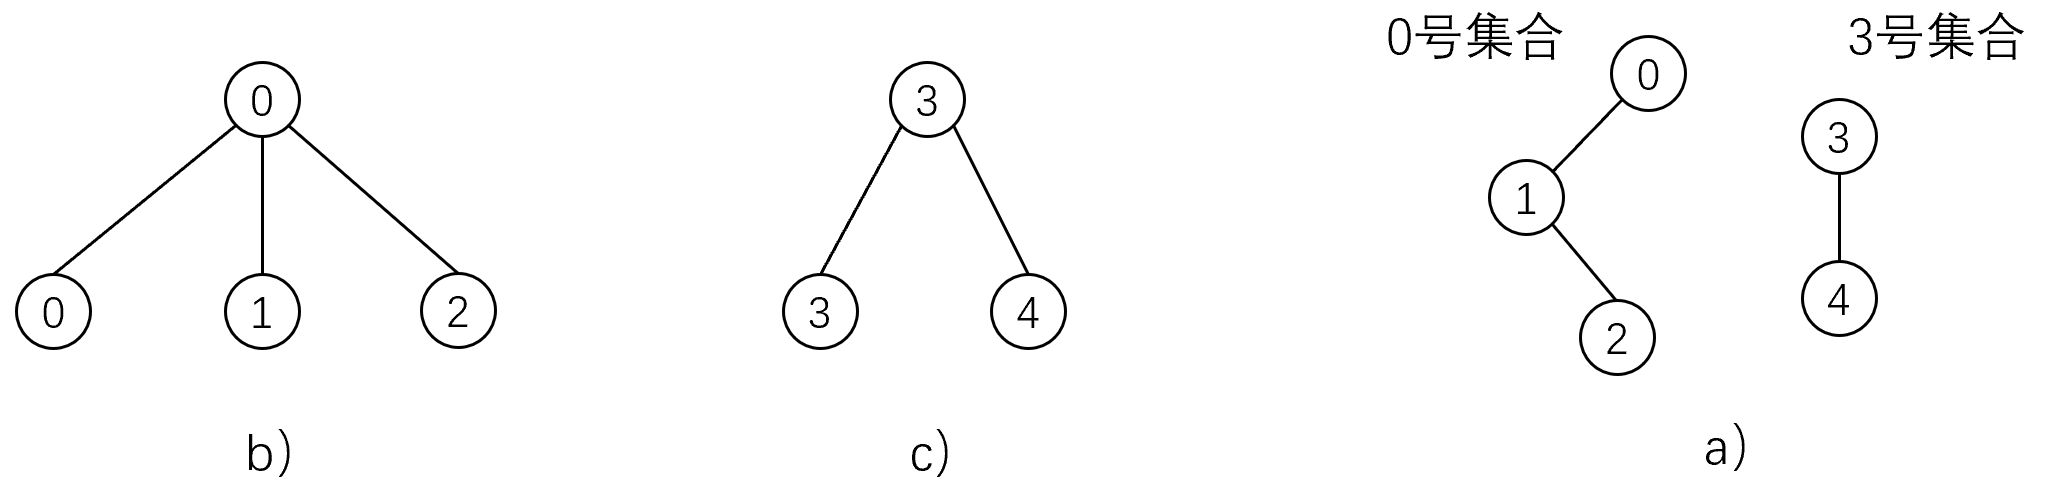
\includegraphics[width=0.80\textwidth]{assets/pics_and_ppts/ch4/并查集思路推导图1.png}    
\end{center}
0、1、2这三个元素属于0号集合，可以认为它们处在根节点为0的树中，如b）；3、4这两个元素属于3号集合，可以认为它们处在根节点为3的树中，如c）。
查找某元素所属集合的过程，就是向上找其根节点的过程；而合并过程实际上是将3和4这两个元素重新“挂在了0上面”，如下图：
\begin{center}
    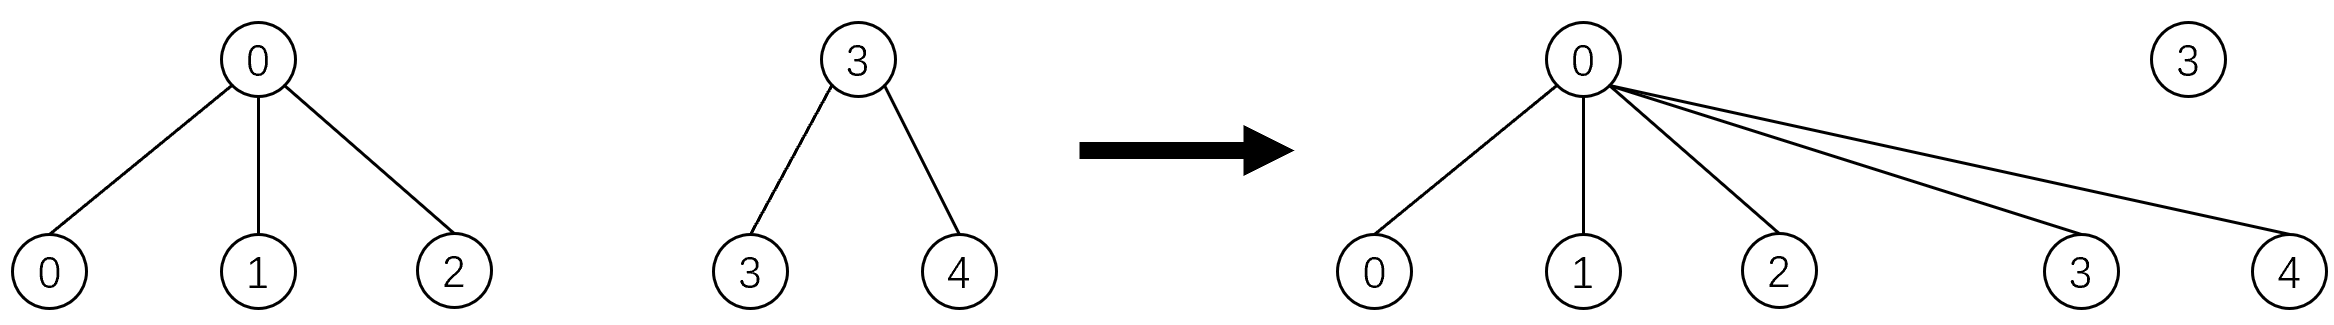
\includegraphics[width=0.85\textwidth]{assets/pics_and_ppts/ch4/并查集思路推导图2.png}    
\end{center}
这样，若是3号集合有十万个元素，就需要更改十万次。

说到这，你想到了什么更好的做法吗？\\

此处应该有留白......\\

没错，如果我们直接将3号集合的根节点3挂在0号集合的根节点0之下，则无论3号集合有多少元素，合并时均只需要一次操作即可实现，如图\ref{fig:并查集思路推导图3}所示：
\begin{figure}[htbp]
    \centering
    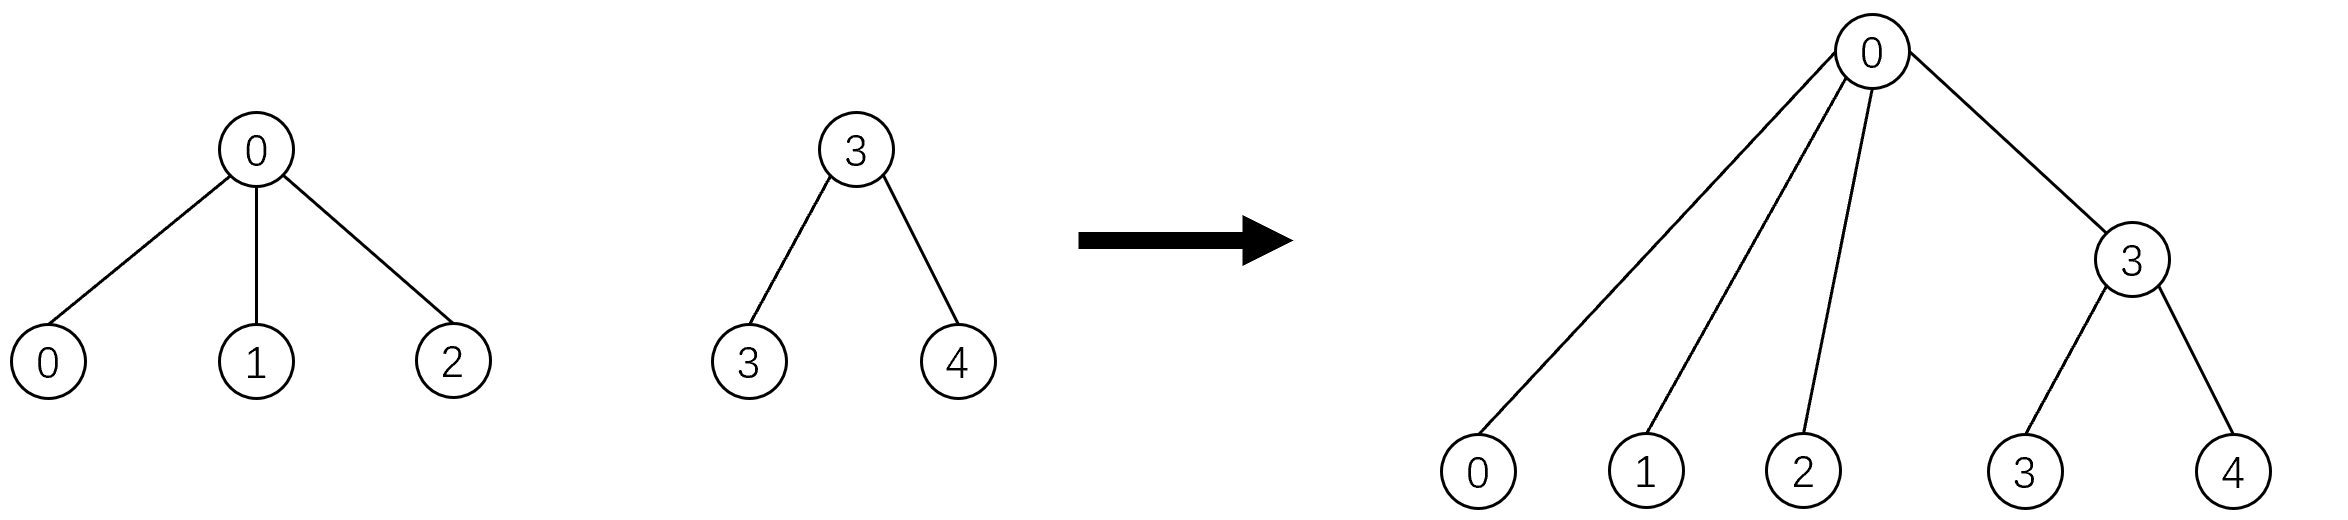
\includegraphics[width=0.87\textwidth]{assets/pics_and_ppts/ch4/并查集思路推导图3.png}
    \caption{}
    \label{fig:并查集思路推导图3}
\end{figure}
并且当我们要查询3、4号节点所属的集合编号时，只需要向上找两次父节点即可，依然可以较为高效地实现。这种用树形结构表示集合，
并通过维护节点之间的父子关系来实现集合合并与查询的数据结构，我们将其称之为\term{并查集（Union-Find）}，这个名字生动地表达了它的功能：并（Union）
和查（Find）。

\textbf{显然，并查集由若干棵树组成，每棵树的根节点编号表示该树中所有元素所处的集合编号。要查询某节点所在集合，只需要顺着树向上找到根节点即可。而合并
操作，仅需将一个集合的根节点作为另一个集合根节点的孩子即可。}

并查集最常见的实现方式是通过一个数组实现：
\begin{cppcode}
    int father[N];
\end{cppcode}
father[i]的值为j就表示元素i在树中的\uline{父}节点为j。若father[i] == i成立，则表示i是这棵树的\uline{根}节点，也即是该集合的编号。比如图\ref{fig:并查集思路推导图3}合并后的图
中有：
\begin{bulk}
    father[0] = 0; \;\; father[1] = 0; \;\; father[2] = 0; \;\;
    father[3] = 3; \;\; father[4] = 3;
\end{bulk}


这样，若最初$N$个城镇分别属于$N$个不同集合，则可以做如下初始化：
\begin{cppcode}
    for(int i=0; i<N; i++) {
        father[i] = i;
    }
\end{cppcode}
在这种设计下，查找和合并操作是非常容易实现的：
\begin{cppcode}
    // 查找操作：查找元素x所属的集合编号ret
    int Find(int father[], int x) {
        int ret = x;
        while(father[ret] != ret) {
            ret = father[ret];
        }
        return ret;
    }
    // 合并操作：若x与y不属于同一个集合，将它们所属的集合合并
    int Union(int father[], int x, int y) {
        int x_id = Find(father, x); // x所属集合的id
        int y_id = Find(father, y); // y所属集合的id
        if(x_id != y_id) {
            father[x_id] = y_id;
            return 1;
        }
        return 0;
    }
\end{cppcode}

\subsection{路径压缩}
随着合并次数的增加，树的层数可能越来越高，则查找每个元素的根节点时开销可能越来越大。因此我们可以在合适的时机对树进行调整，将每个元素跳过所有
父节点而直接指向根节点，如下图：
\begin{center}
    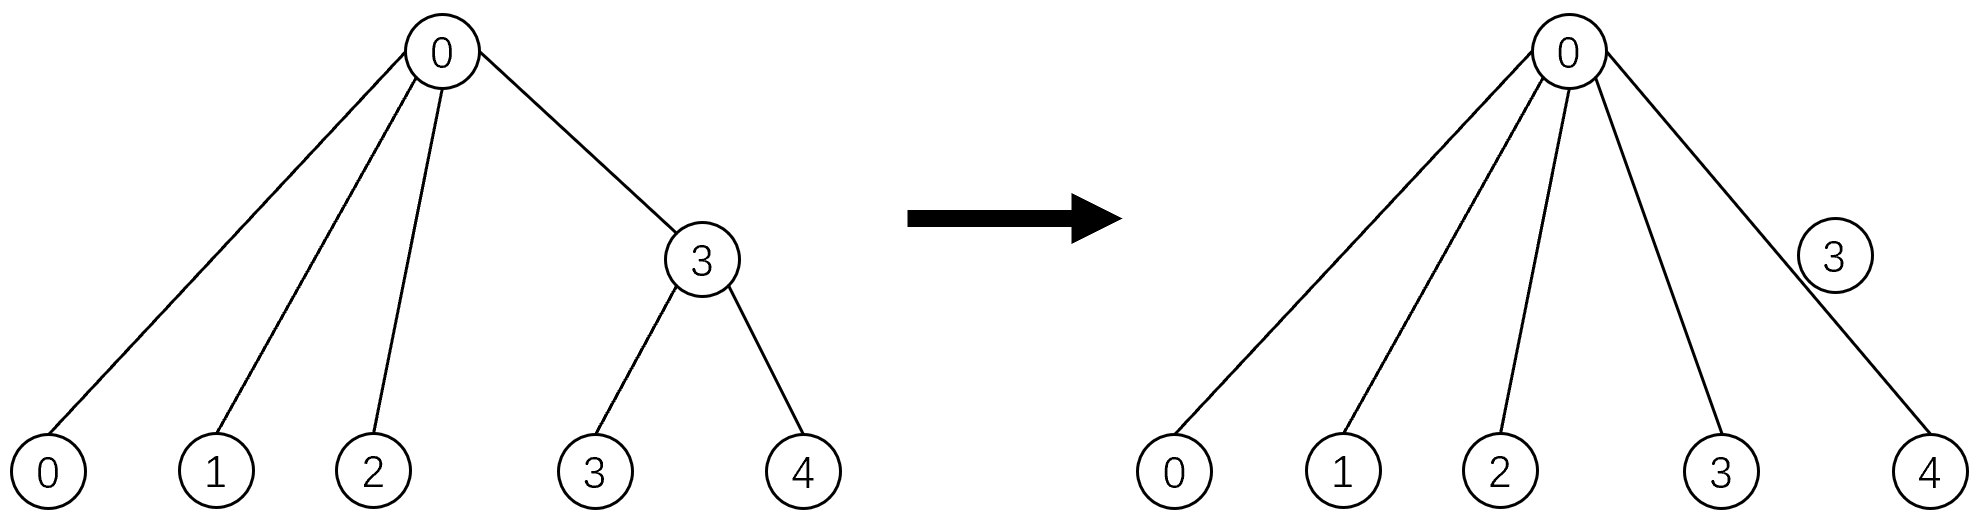
\includegraphics[width=0.82\textwidth]{assets/pics_and_ppts/ch4/并查集路径压缩优化示意.png}
\end{center}

这种优化策略被称为\term{路径压缩}。
显然查找元素（Find）时，会一路向上找到根节点，因此在Find时顺手对路径上所有进行调整是非常合适的。此外，
路径压缩不仅可以出现在独立的 Find 操作中，也会在 Union 调用 Find 时自动发生。因此，路径压缩不需要在 Union 中额外重复实现。

带路径压缩的Find函数代码如下：

\begin{cppcode}
    // 查找元素x所属的集合编号
    int Find(int father[], int x) {
        int ret = x;
        while(father[ret] != ret) {
            ret = father[ret];
        }
        // 路径压缩，将x到ret路径上的所有节点的father[]均指向ret
        int to_adjust = x;
        while(to_adjust != ret) {
            int fa = father[to_adjust];
            father[to_adjust] = ret;
            to_adjust = fa;
        }
        return ret;
    }
\end{cppcode}

\subsection{*按秩合并}
事实上很多人可能想到了，在合并两棵树时，将高度更小的树挂在高度更大的树下面一定是更好的，这样查找路径会更短。可是对于带路径压缩的并查集，我们难以对树的高度
进行准确的维护。因此，我们对每棵树记录一个数值，表示它“最大达到过多高”，这个数值称为\term{秩}。

初始时每棵树只有一个节点，因此秩为 1。合并两棵树时：\\
1）如果两棵树的秩不同，就将秩较小的树挂到秩较大的树下面，新树的秩保持不变。\\
2）如果两棵树的秩相同，就任选一棵树作为新树的根节点，另一棵树挂到它下面，新树的秩增加 1。

需要注意的是，秩并不一定等于树当前的实际高度。在不使用路径压缩时，按照上述规则，秩等于树的高度；引入路径压缩后，树的实际高度可能下降，但秩不会随之减小。
因此秩不是一个精确的指标，而是一个足以支持正确决策、同时又容易维护的指标。

我们通过一个rank[]数组记录树的秩，rank[i]表示元素i所在的树的秩。按秩合并的Uinon函数实现如下：
\begin{cppcode}
    // 若x与y不属于同一个集合，将它们所属的集合合并
    int Union(int father[], int rank[], int x, int y) {
        int x_id = Find(father, x); // x所属集合的根节点
        int y_id = Find(father, y); // y所属集合的根节点

        if(x_id != y_id) {
            // x所在的树秩更小
            if(rank[x_id] < rank[y_id]) {
                father[x_id] = y_id;
            } 
            // y所在的树秩更小
            else if(rank[x_id] > rank[y_id]) {
                father[y_id] = x_id;
            } 
            // 两棵树秩相等
            else {
                father[x_id] = y_id;
                rank[y_id]++;
            }
            return 1;
        }
        return 0;
    }
\end{cppcode}
在Find函数中实现路径压缩、在Uinon函数中实现按秩合并，通常可以让并查集始终保持较高效的合并、查找。关于并查集相关操作具体的复杂度分析较为复杂，
感兴趣的话请大家参考相关资料。

\clearpage%%%%%%%%%%%%%%%%%%%%%%%%%%%%%%%%%%%%%%%%%%%%%%%%%%%%%%%%%%%%%%%%%%%%%%%%%%%%%%%%%%%%%%%%%%%%%%%%%%%%%%%%%%%%%%%%%%%%%%%%%%%%%%%%%%%%%%%%%%%%%
\begin{exercise}
    1. 若某哈夫曼树度为2的节点有7个，能否确定度为0的节点有几个？\\

    2. 若某哈夫曼树度为2的节点有7个，能否确定这棵哈夫曼树共有几个节点？\\

    3. 练习：有5个元素A、B、C、D、E的权值分别为1,2,2,4,5，将这五个元素作为叶节点构造一棵哈夫曼树。\\

    4. 下列完全二叉树中，是最小堆的有\underline{\hspace{1.5cm}}，是最大堆的有\underline{\hspace{1.5cm}}。\\[0.5em]
    \begin{center}
        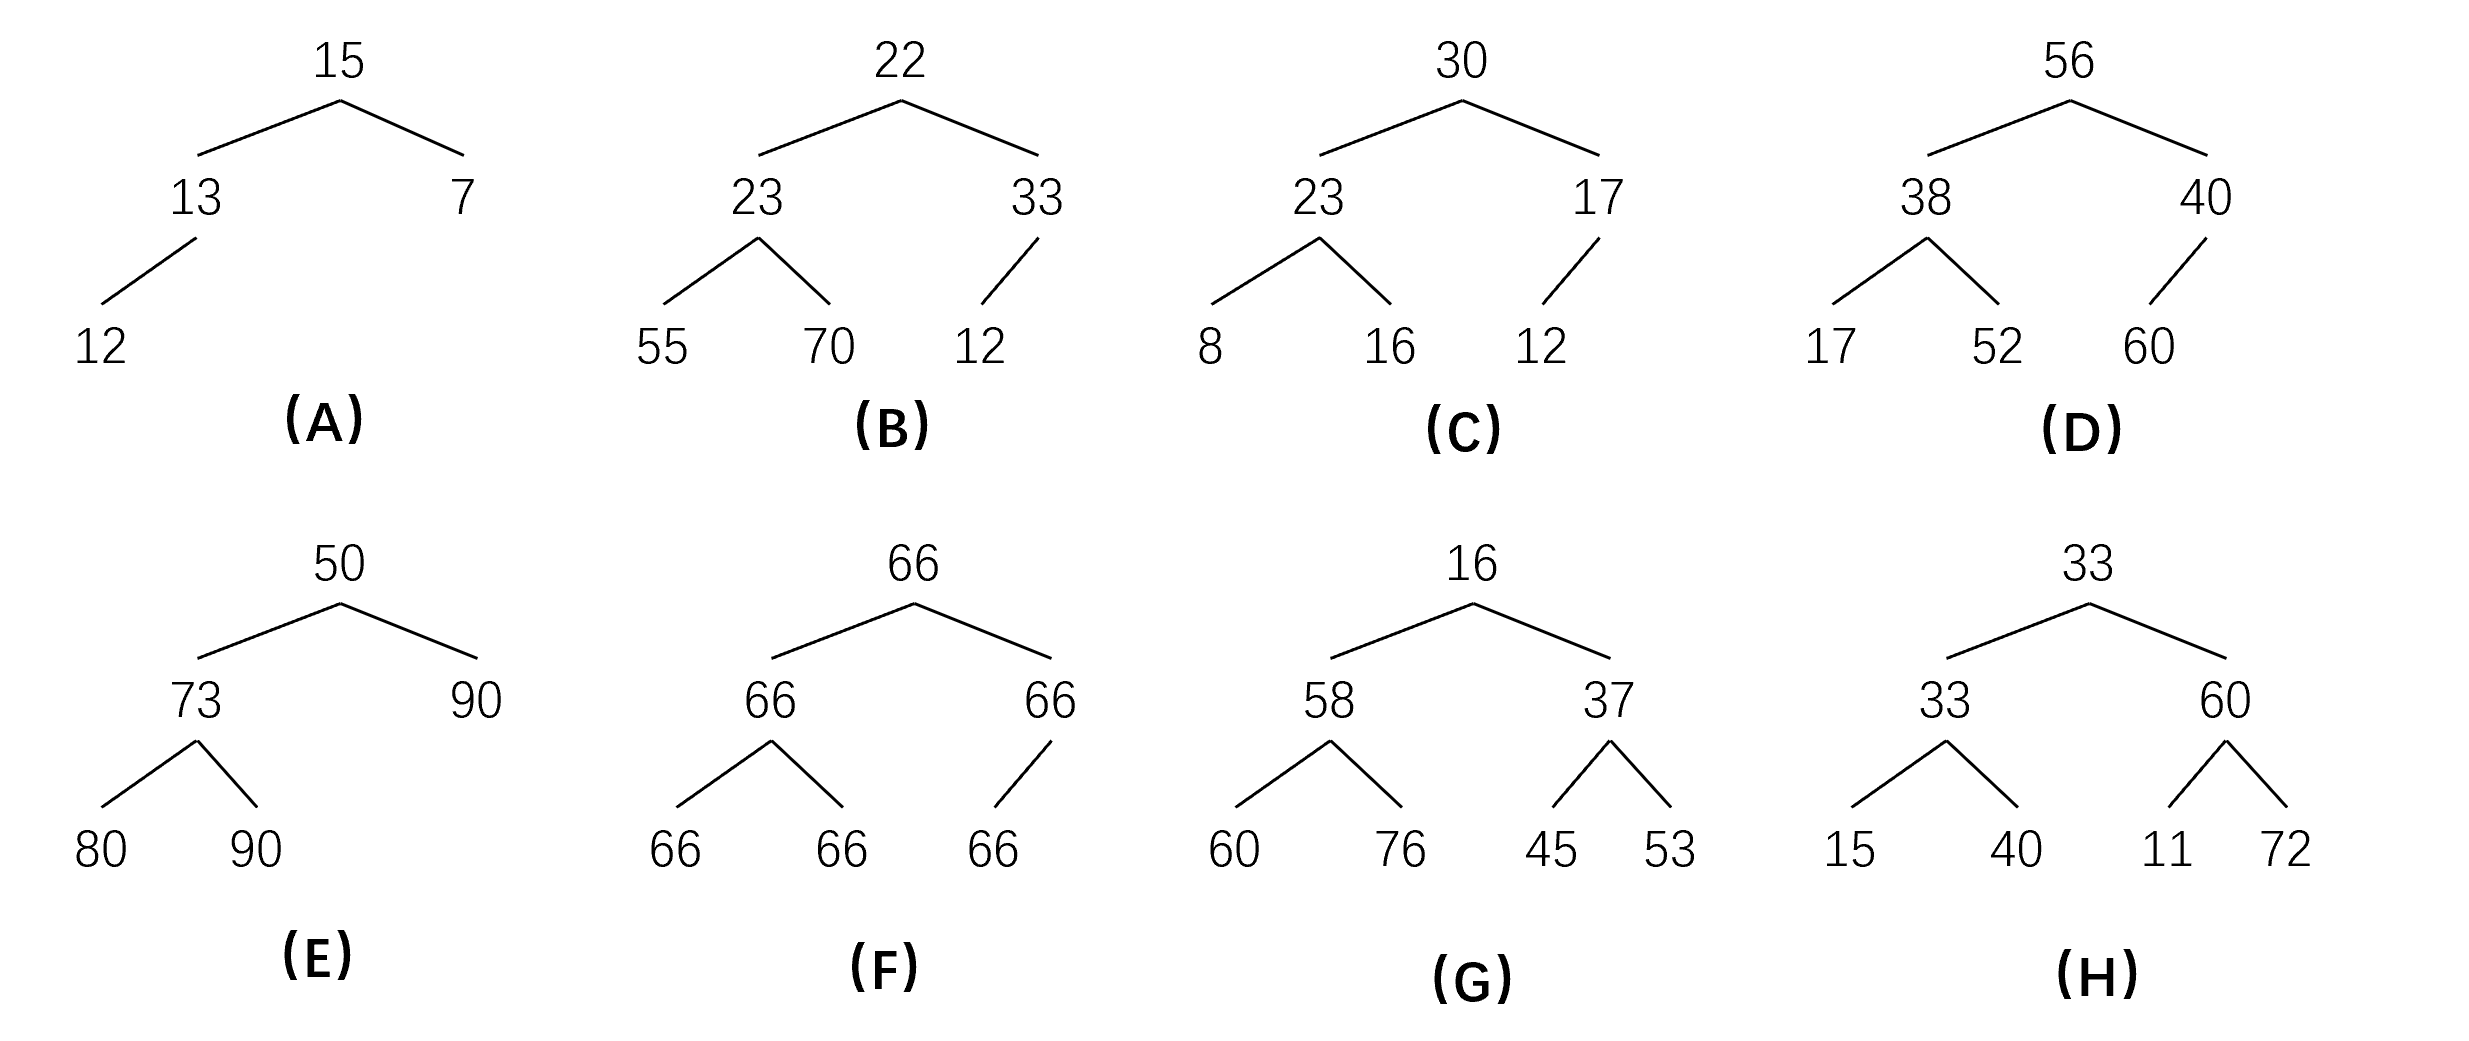
\includegraphics[width=0.88\textwidth]{assets/pics_and_ppts/ch4/习题_判断最大堆和最小堆.png}
    \end{center}

    5. 对于下图所示的二叉树，各节点中的数字表示该节点的权值。下列说法错误的是\underline{\hspace{1cm}}\\[0.5em]
    \begin{center}
        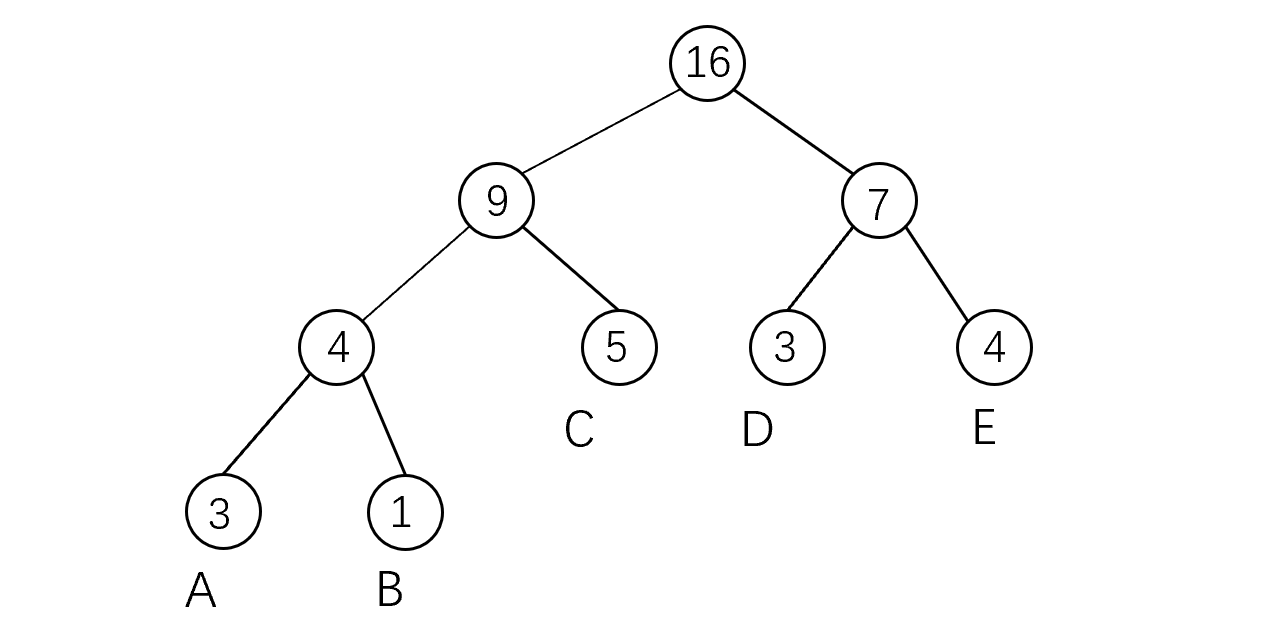
\includegraphics[width=0.57\textwidth]{assets/pics_and_ppts/ch4/习题图_一棵哈夫曼树.png}
    \end{center}

\noindent A. 节点B的带权路径长度为3\\
B. 这棵树的带权路径长度为60\\
C. 以A、B、C、D、E为叶节点构造一棵二叉树，图示的树能使得带权路径长度达到最小\\
D. 以A、B、C、D、E为叶节点构造一棵二叉树，图示的树并不是唯一的带权路径长度最小的树\\

    6. C++标准库已经封装好了一个数据结构：priority\_queue，这是一个最小堆，可以通过：
    \begin{bulk}
        priority\_queue<int, vector<int>, greater<int> > min\_heap;            
    \end{bulk}
    定义并初始化一个初始为空的，名为min\_heap的最小堆，可容纳int类型元素。其中
    \begin{bulk}
        priority\_queue<int, vector<int>, greater<int> >
    \end{bulk}
    是一种类型，只不过看起来比较长而已。读者大可不必关注其细节，只知道上述代码用该类型定义的min\_heap是一个最小堆，并直接使用相关操作即可。
    min\_heap支持以下操作：
    \begin{enumerate}[label=\arabic*）]
        \item min\_heap.push(e);  // 向堆中插入一个值为e的元素；
        \item int a = min\_heap.top();   // 获取堆顶元素，赋值给a(但不删除堆顶元素)；
        \item min\_heap.pop();       // 删除堆顶元素；
        \item min\_heap.size();      // 返回堆中元素数量；
        \item min\_heap.empty();     // 若堆为空，返回true，否则返回false。
    \end{enumerate}
    对初始为空的minHeap依次执行以下操作，请指出每一次使用min\_heap.top()获取堆顶元素时，获取到的元素值是多少。
    \begin{enumerate}[label=\arabic*）]
        \item min\_heap.push(5);  
        \item min\_heap.top();    // 1
        \item min\_heap.push(3);
        \item min\_heap.push(4);  
        \item min\_heap.top();    // 2
        \item min\_heap.pop();    
        \item min\_heap.top();    // 3
    \end{enumerate}

    \vspace{\baselineskip}

    7. 请你借助{\color{red}\textbf{上题}}给出的priority\_queue及其相关操作来解决“合并柴薪”问题。输入一个长度为n的数组w[]表示各堆柴薪的重量（均为正整数），返回一个正整数，
    表示最优情况下消耗的体力值。
    \begin{cppcode}
        int MinCost(int w[], int n) {
            priority_queue<int, vector<int>, greater<int>> min_heap;      
            // 在下方完成你的代码
        }
    \end{cppcode}

    8. （某年408真题）对n个互不相同的符号进行哈夫曼编码，若生成的哈夫曼树共有115个节点，则n的值是\\[0.5em]
    \begin{tabular}{llll}
    A. 56 & B. 57 & C. 58 & D. 60
    \end{tabular}\\

    9. （某年408真题）若某二叉树有5个叶节点，其权值分别为10，12，16，21，30，则其最小的带权路径长度（WPL）是\underline{\hspace{1cm}}\\[0.5em]
    \begin{tabular}{llll}
        A. 89 & B. 200 & C. 208 & D. 289
    \end{tabular}\\
    

    10. 请你实现一个算法，求使用二叉链表存储的二叉树的带权路径长度。空树直接返回0。
    \begin{cppcode}
        struct node {
            // int data;  本题仅节点权重有意义，数据可忽略
            int weight;
            node* lchild; 
            node* rchild; 
        };
    \end{cppcode}
    注意：二叉树的带权路径长度（WPL）定义为所有叶节点的带权路径长度之和，非叶节点不参与计算。

    \vspace{\baselineskip}

    11. 某大陆散布着多个地下遗迹，这些地下遗迹都可以被建模成一棵二叉树，根节点为遗迹的入口，向下探索，每个节点代表一个房间，所有处于叶节点的房间都能挖出
    宝藏，weight(weight>0)表示宝藏的价值。由于遗迹深处的宝藏获取难度更大，某位名为CoreLoop的探险者决定权衡风险与收益，
     $\frac{1}{\text{节点深度}}*\text{宝藏价值}$ 定义为房间的“诱人值”。请你实现一个算法，帮CoreLoop算出二叉树T中诱人值最大的房间诱
     人值是多少。（根节点深度定义为1；空树诱人值定义为0）。
    \begin{cppcode}
        double CalcAppeal(node* T) {
            double ans = 0;
            // your codes...

            return ans;
        }
    \end{cppcode}
    二叉树的节点定义{\color{red}\textbf{同上一题所示}}。你完全可以实现其他函数，并在CalcAppeal中调用。\\

    12. 某位名为CoreLoop的探险者误入了一扇魔法门从而被传送到了一片地底世界，他只能通过前方的地下城回到大陆。该地下城可以被建模为一棵
    二叉树，每个节点代表一个房间，根节点表示入口，也是必须经过的房间。节点的 weight(weight>0) 表示进入该房间所需消耗的能量，叶节点代表所有可以回到大陆的
    出口。CoreLoop可以沿任何一条路径经出口走出地下城。请你实现一个算法帮助CoreLoop求出最优路径（消耗能量最小）下，逃离地下城需要消耗的能量值。root保证不是空树。
    \begin{cppcode}
        struct node {
            int weight;     // 进入房间需要消耗的能量
            node* lchild; 
            node* rchild; 
        };
        int MinEscapeCost(node* root) {
            
        }
    \end{cppcode}
    

\end{exercise}
\clearpage

\begin{exerciseanswer}
    1. 答：能确定度为0的节点有8个。哈夫曼树一定是二叉树，因此根据$n_0=n_2+1$，度为0的节点有 7 + 1 = 8个。\\

    2. 答：能确定哈夫曼树共有15个节点。由前面的讨论（参见哈夫曼树的性质，第\pageref{minisec:哈夫曼树的性质}页）可知，哈夫曼树中不存在度为1的节点，因此总节点数
    $n = n_0 + n_1 + n_2 = n_0 + n_2 = 7 + 8 = 15$。\\

    3. 略。\\

    4. 最小堆有：E、F、G；最大堆有：A、C、F。\\

    5. 选B。节点B的带权路径长度为3*1 = 3，A正确；树的带权路径长度是所有叶节点的带权路径长度之和：3*(3+1) + 2*(5+3+4) = 12 + 24 = 36，B错误；C、D显然正确。\\

    6. 显然，本题我们只要关注堆顶元素（即最小的那一个）是什么即可：
    \begin{enumerate}[label=\arabic*）]
        \item min\_heap.push(5);  // 堆中元素：5；堆顶为5
        \item min\_heap.top();    // 获取到的为5
        \item min\_heap.push(3);  // 堆中元素：5、3；堆顶为3
        \item min\_heap.push(4);  // 堆中元素：5、3、4，堆顶为3
        \item min\_heap.top();    // 获取到的为3
        \item min\_heap.pop();    // 删除堆顶元素3，4成为新的堆顶
        \item min\_heap.top();    // 获取到的为4
    \end{enumerate}

    \vspace{\baselineskip}

    7. 每次在堆中选出两个最小的来合并，计算相应体力消耗，并将合并后的新柴薪加入堆中。做n-1次即可。
    \begin{cppcode}
        int MinCost(int w[], int n) {
            priority_queue<int, vector<int>, greater<int>> min_heap;      
            // 在下方完成你的代码
            int total_cost = 0;
            
            for(int i=0; i<n; i++) {
                min_heap.push(w[i]);
            }
            // 做n-1次
            for(int i=1; i<=n-1; i++) {
                // 取出两个重量最小的：w1和w2
                int w1 = min_heap.top();
                min_heap.pop();
                int w2 = min_heap.top();
                min_heap.pop();

                // 体力消耗为w1+w2
                int union_cost = w1 + w2;
                total_cost += union_cost;
                
                // 合成一堆后放回堆中
                min_heap.push(union_cost);
            }
            return total_cost;
        }
    \end{cppcode}

    \vspace{\baselineskip}

    8. 选C。哈夫曼编码，被编码的符号一定都是叶节点，又：哈夫曼树中没有只有叶节点和度为2的节点，因此有: $n_0+n_2=n_2+1+n_2=115$，得$n_2=57, n_0=58$。
    
    另外一种理解，生成哈夫曼树，需要合并n-1次，因此生成的度为2的节点为n-1个，代入计算也可。\\

    9. 选B。可以构造如下图所示的哈夫曼树。求出带权路径长度WPL=3*(10+12) + 2*(30+16+12) = 200。
    \begin{center}
        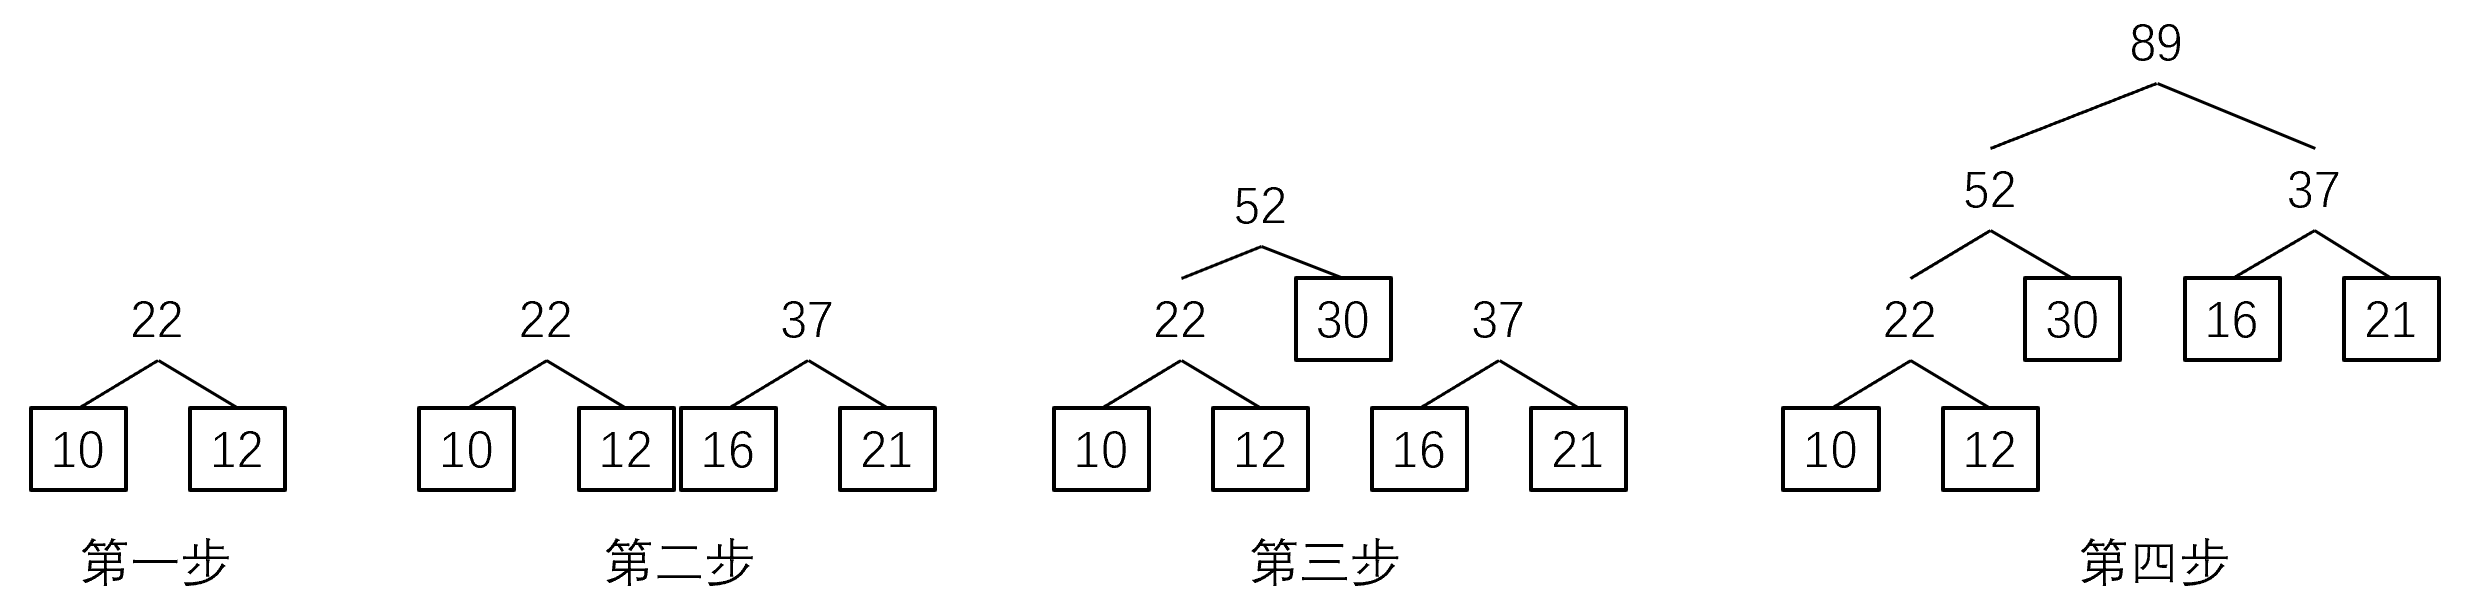
\includegraphics[width=0.89\textwidth]{assets/pics_and_ppts/ch4/21408_哈夫曼树构造过程.png}
    \end{center}

    \vspace{\baselineskip}

    10. 本题可以记录一个变量total，递归地访问每一个节点，将所有访问到的叶节点的带权路径长度累加记录，最终total的值就是树的带权路径长度WPL。这里我们给出另一种
    思路的实现代码：
    
    不难发现，每棵子树T的WPL等于其左子树与右子树的WPL之和。因此求T的WPL，可以递归地转化为求T->lchild以及T->rchild的WPL。递归边界就是左子树或右子树为空树。
    代码如下所示。
    \begin{cppcode}
        int WPL(node* root, int depth) {
            // 空树，直接返回0
            if(root == NULL) return 0;
            // 当前递归到的，以root为根节点的子树，其左右子树都是空树，因此root的WPL可以直接计算。
            if(root->lchild == NULL && root->rchild == NULL) {
                return root->weight * (depth-1);    // 深度为depth的节点，根节点到其路径长度为depth-1
            }
            // root还有子树，需要递归地计算子树的WPL并加到一起，作为root的WPL返回
            int total = 0;    
            if(root->lchild != NULL) {
                total += WPL(root->lchild, depth+1);
            }
            if(root->rchild != NULL) {
                total += WPL(root->rchild, depth+1);
            }

            return total;
        }
    \end{cppcode}
    调用WPL(T, 1)即可求出T的带权路径长度。注意：我们这里按照惯例，将根节点深度定义成了1，这恰好能正确处理“只有一个根节点的树”的情况。\\

    11. 实际上本题依然是通过叶节点的深度和权值计算出叶结点的“诱人值”，可以看成某种“特殊的带权路径长度”，只不过求WPL是累加，而本题是“记录最大”。我们可以通过一个引用变量（或指针）记录
    递归过程中的最大值，代码如下：
    \begin{cppcode}
    
        void visit(node* root, int depth, double& max_appeal) {
            if(root == NULL) return ;

            // 叶子节点，有宝藏的房间
            if(root->lchild == NULL && root->rchild == NULL) {
                double appeal = (1.0/dpeth) * root->weight;
                // 本房间的“诱人值”比之前遇到的所有房间都大，更新max_appeal
                if(appeal > max_appeal) {
                    max_appeal = appeal;
                }
            }
            if(root->lchild != NULL) {
                visit(root->lchild, depth+1, max_appeal);
            }
            if(root->rchild != NULL) {
                visit(root->rchild, depth+1, max_appeal);
            }
            
        }
        
        double CalcAppeal(node* T) {
            double ans = 0;
            // your codes...
            visit(T, 1, ans);
            return ans;
        }
    \end{cppcode}
    \vspace{\baselineskip}

    12. 本题的核心思想在于，对于以节点u为起点的逃生路线有：
    \[
        MinCost(u)=weight(u)+\min(MinCost(left),MinCost(right))
    \]
    left、right分别表示u的左右子树。想通了这一点，题目就变得非常简单。请参见代码与注释。
    \begin{cppcode}
        int MinEscapeCost(node* root) {
            if(root == NULL) return 0;

            // 叶子节点，出口找到了 
            if(root->lchild == NULL && root->rchild == NULL) {
                return root->weight;
            }
            // 左边是死路，只能从右边走
            if(root->lchild == NULL) {
                return root->weight + MinEscapeCost(root->rchild);
            }
            // 右边是死路
            if(root->rchild == NULL) {
                return root->weight + MinEscapeCost(root->lchild);
            }

            // 两边都能走，递归计算两边代价后，选代价小的那一条路
            int ltree_cost = MinEscapeCost(root->lchild);
            int rtree_cost = MinEscapeCost(root->rchild);

            return root->weight + min(ltree_cost, rtree_cost);
        }
    \end{cppcode}
    \vspace{\baselineskip}

\end{exerciseanswer}%%%%%%%%%%%%%%%%%%%%%%%%%%%%%%%%%%%%%%%%%%%%%%%%%%%%%%%%%%%%%%%%%%%%%%%%%%%%%%%%%%%%%%%%%%%%%%%%%%%%%%%%%%%%%%%%%%%%%%%%%%%%%%%%



